% Autor: Francisco Javier Barranco Tena
% Apendice con los resultados de los experimentos realizados en el desarrollo del TFG
% Alt + z o Option + z para activar el word wrap en Visual Studio Code

\section{Experimento 1: Entrenamiento con datos de Estados Unidos y validación cruzada}
En la figura \ref{fig:exp1_val_output} se pueden ver los resultados de la validación de los modelos en cada iteración del experimento 1. En la sección \ref{SEC:EXP1} se ha explicado en detalle cómo se ha llevado a cabo este experimento y se han mostrado un resumen de los resultados obtenidos en cada iteración. En la tabla \ref{tab:exp1_results} se pueden ver estos resultados.

% Añadimos ../img/exp1-val-output.png
\begin{figure}[H]
    \centering
    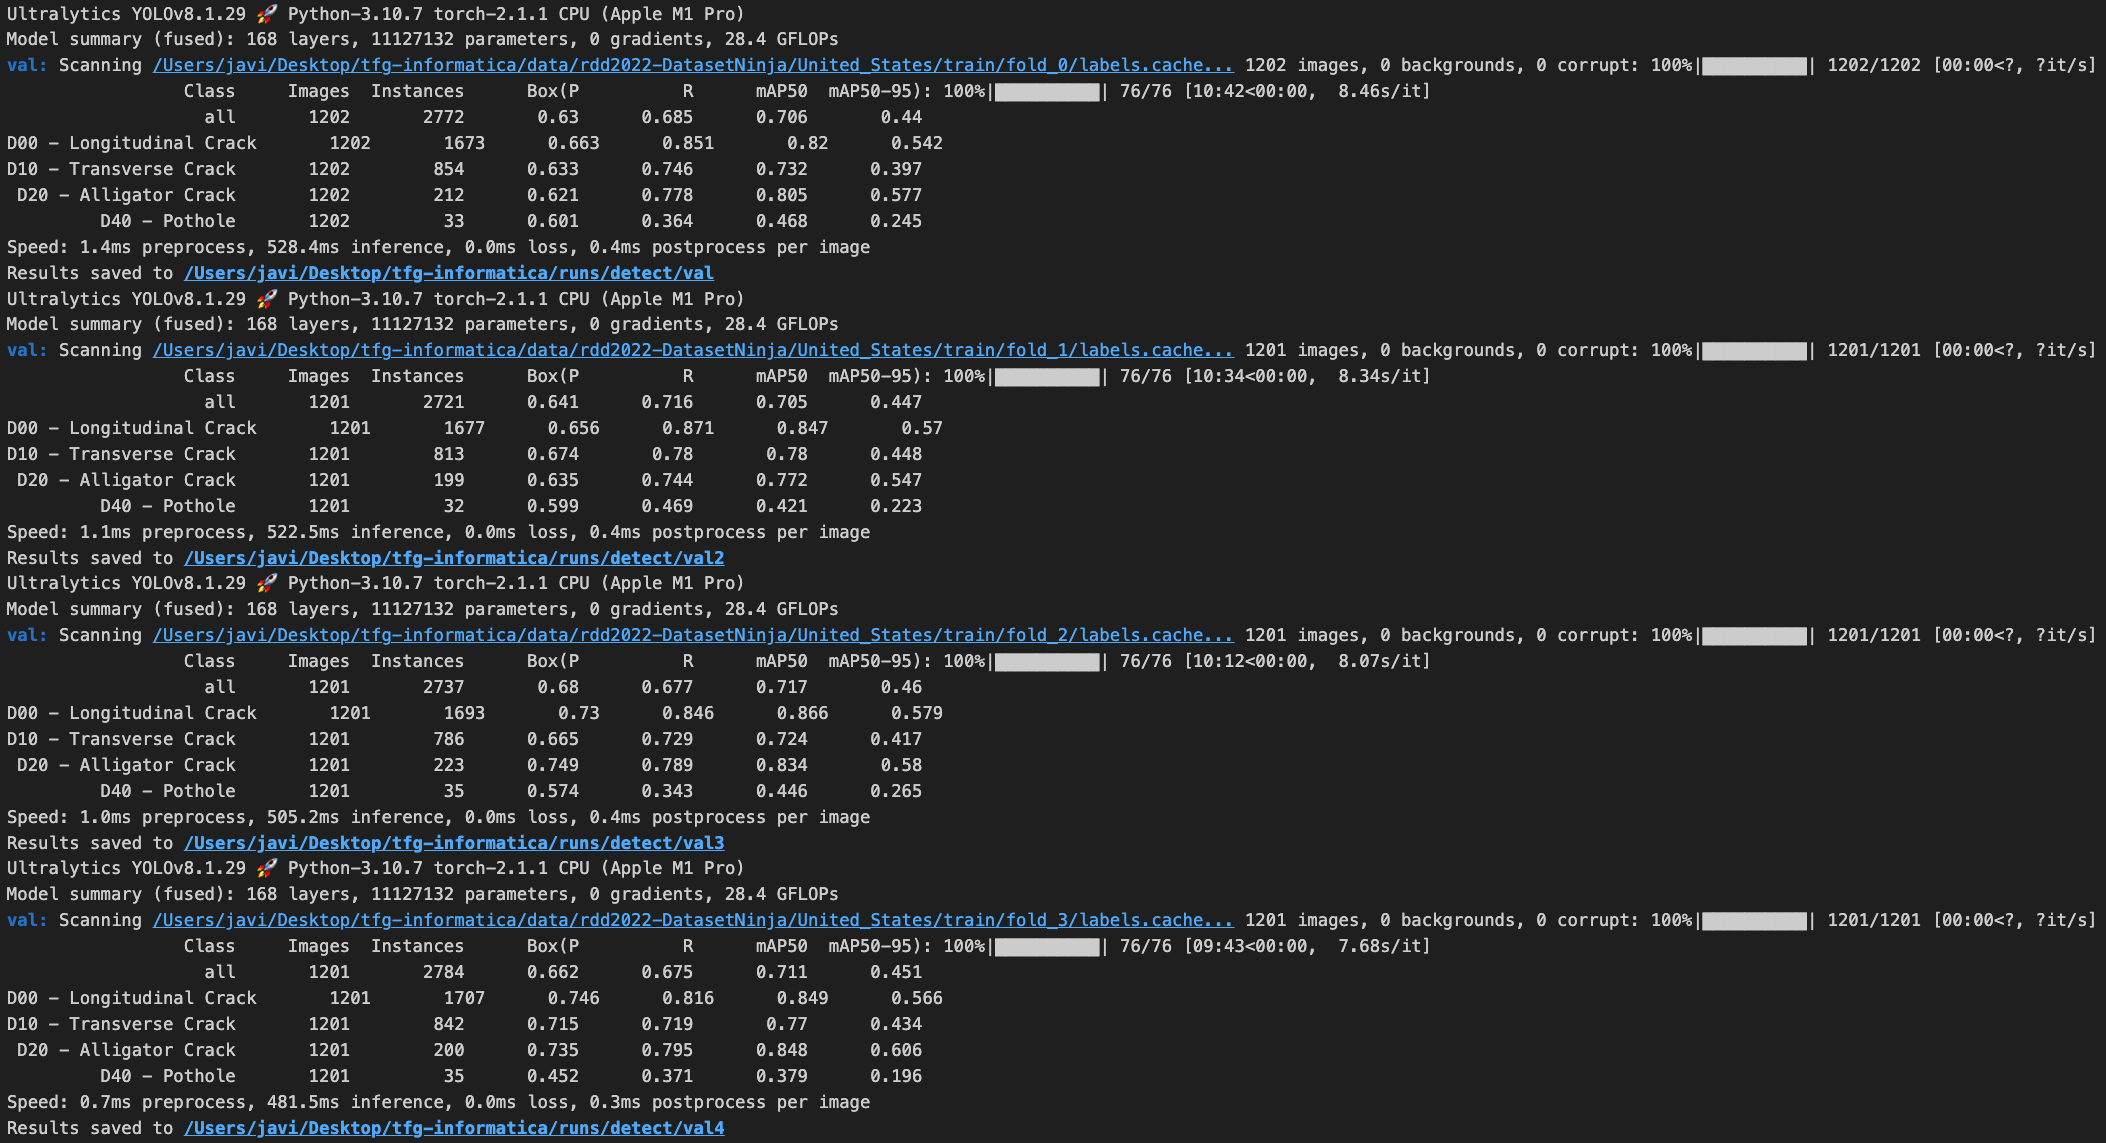
\includegraphics[width=\textwidth,height=\textheight,keepaspectratio]{../img/exp1-val-output.png}
    \caption{Resultados de la validación de los modelos en cada iteración del experimento 1.}
    \label{fig:exp1_val_output}
\end{figure}
\newpage

\section{Experimento 2: YOLOv8 \textit{very large} con todos los datos de Estados Unidos}
En la figura \ref{fig:exp2_val_output} se pueden ver el resultado de la validación del modelo del experimento 2. En este experimento se han entrenado con todos los datos anotados de Estados Unidos y se ha utilizado el fold 0 como conjunto de validación. Es decir, se ha validado con datos que también se han usado en el entrenamiento, por lo que estas metricas no son totalmente fiables. No obstante, como se explica en la sección \ref{SEC:EXP2}, el objetivo de este experimento es comprobar si se puede mejorar el rendimiento del modelo y si se puede obtener un f1-score más alto en la plataforma de la CRDDC2022 usando todos los datos para entrenar y un modelo YOLOv8 de mayor tamaño, en este caso, very large. El resultado del experimento ha sido favorable, ya que se ha subido de un f1-score de 0.515 en el experimento 1 a un f1-score de 0.607 en el experimento 2.

% Añadimos ../img/exp2-val-output.png
\begin{figure}[H]
    \centering
    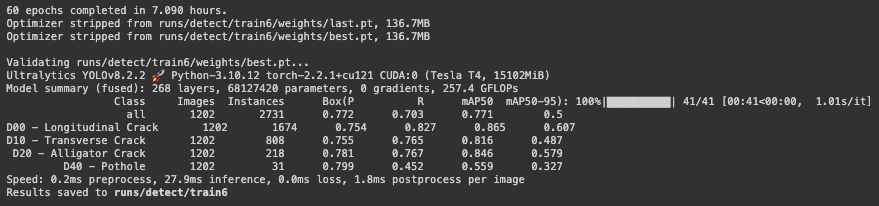
\includegraphics[width=\textwidth,height=\textheight,keepaspectratio]{../img/exp2-val-output.png}
    \caption{Resultados de la validación de los modelos en cada iteración del experimento 2.}
    \label{fig:exp2_val_output}
\end{figure}
\newpage


\section{Experimento 3: Entrenamiento de modelo base con todos los datos de la CRDDC2022}
En la figura \ref{fig:exp3_val_output} se pueden ver los resultados de la validación del modelo del experimento 3 sobre los datos de \textit{fold\_0} de todos los conjuntos de datos, solo India, solo Japon, solo Noruega y solo Estados Unidos respectivamente. 

La figura \ref{fig:exp3_val0_all_confusion_matrices} muestra las matrices de confusión normalizada y sin normalizar de la validación del modelo del experimento 3 sobre los datos de \textit{fold\_0} de todos los datos del conjunto de datos. Las figuras \ref{fig:exp3_val0_confusion_matrices_normalized} y \ref{fig:exp3_val0_confusion_matrices} muestran las matrices de confusión normalizadas y sin normalizar de la validación del modelo del experimento 3 sobre los datos de \textit{fold\_0} de India, Japón, Noruega y Estados Unidos respectivamente.

% Añadimos ../img/exp3-val-output.png
\begin{figure}[H]
    \centering
    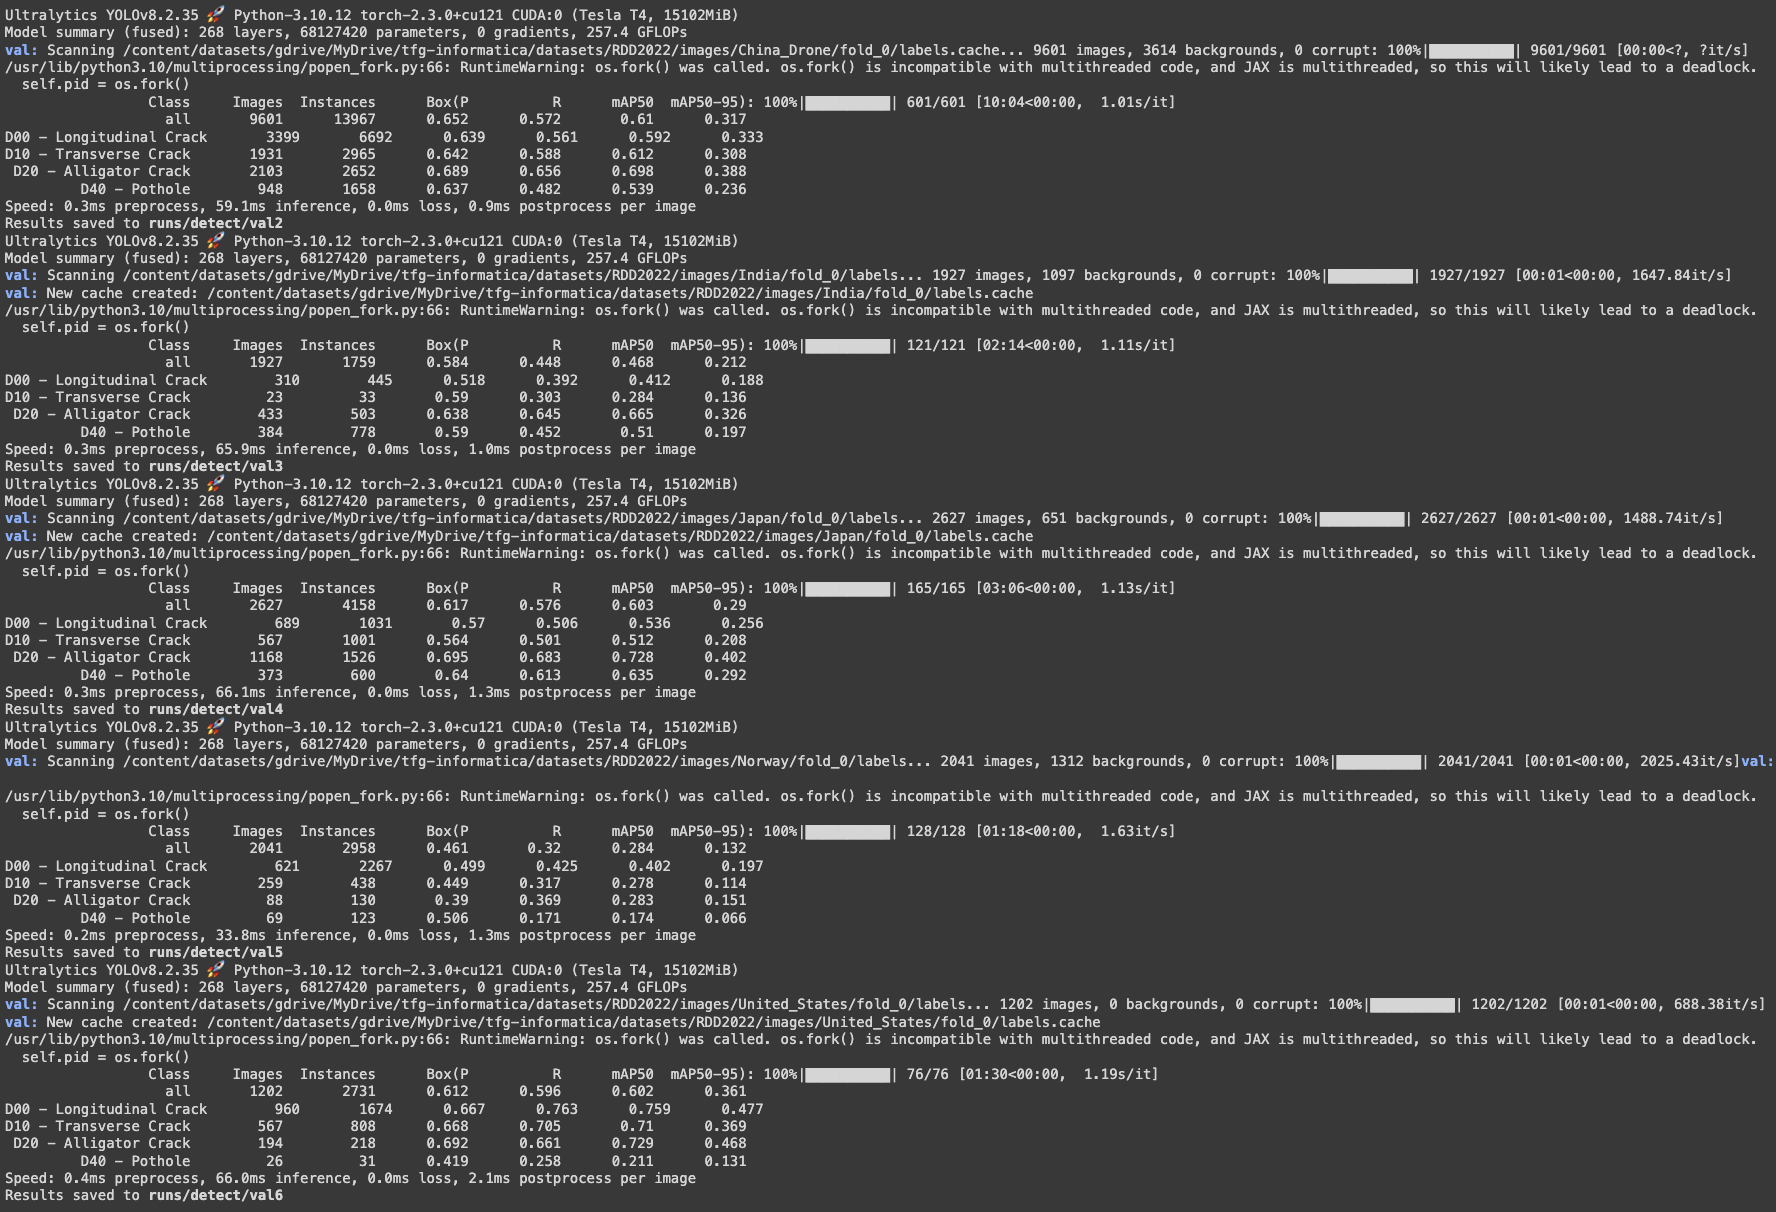
\includegraphics[width=\textwidth,height=\textheight,keepaspectratio]{../img/exp3-val-output.png}
    \caption{Resultados de la validación del modelo del experimento 3 sobre los datos de \textit{fold\_0} de todos los conjuntos de datos, solo India, solo Japon, solo Noruega y solo Estados Unidos respectivamente.}
    \label{fig:exp3_val_output}
\end{figure}
\newpage

% Añadimos ../img/exp3-val0-all-confusion_matrix_normalized.png y ../img/exp3-val0-all-confusion_matrix
\begin{figure}[H]
    \centering
    \subfigure[Matriz de confusión normalizada.]{
        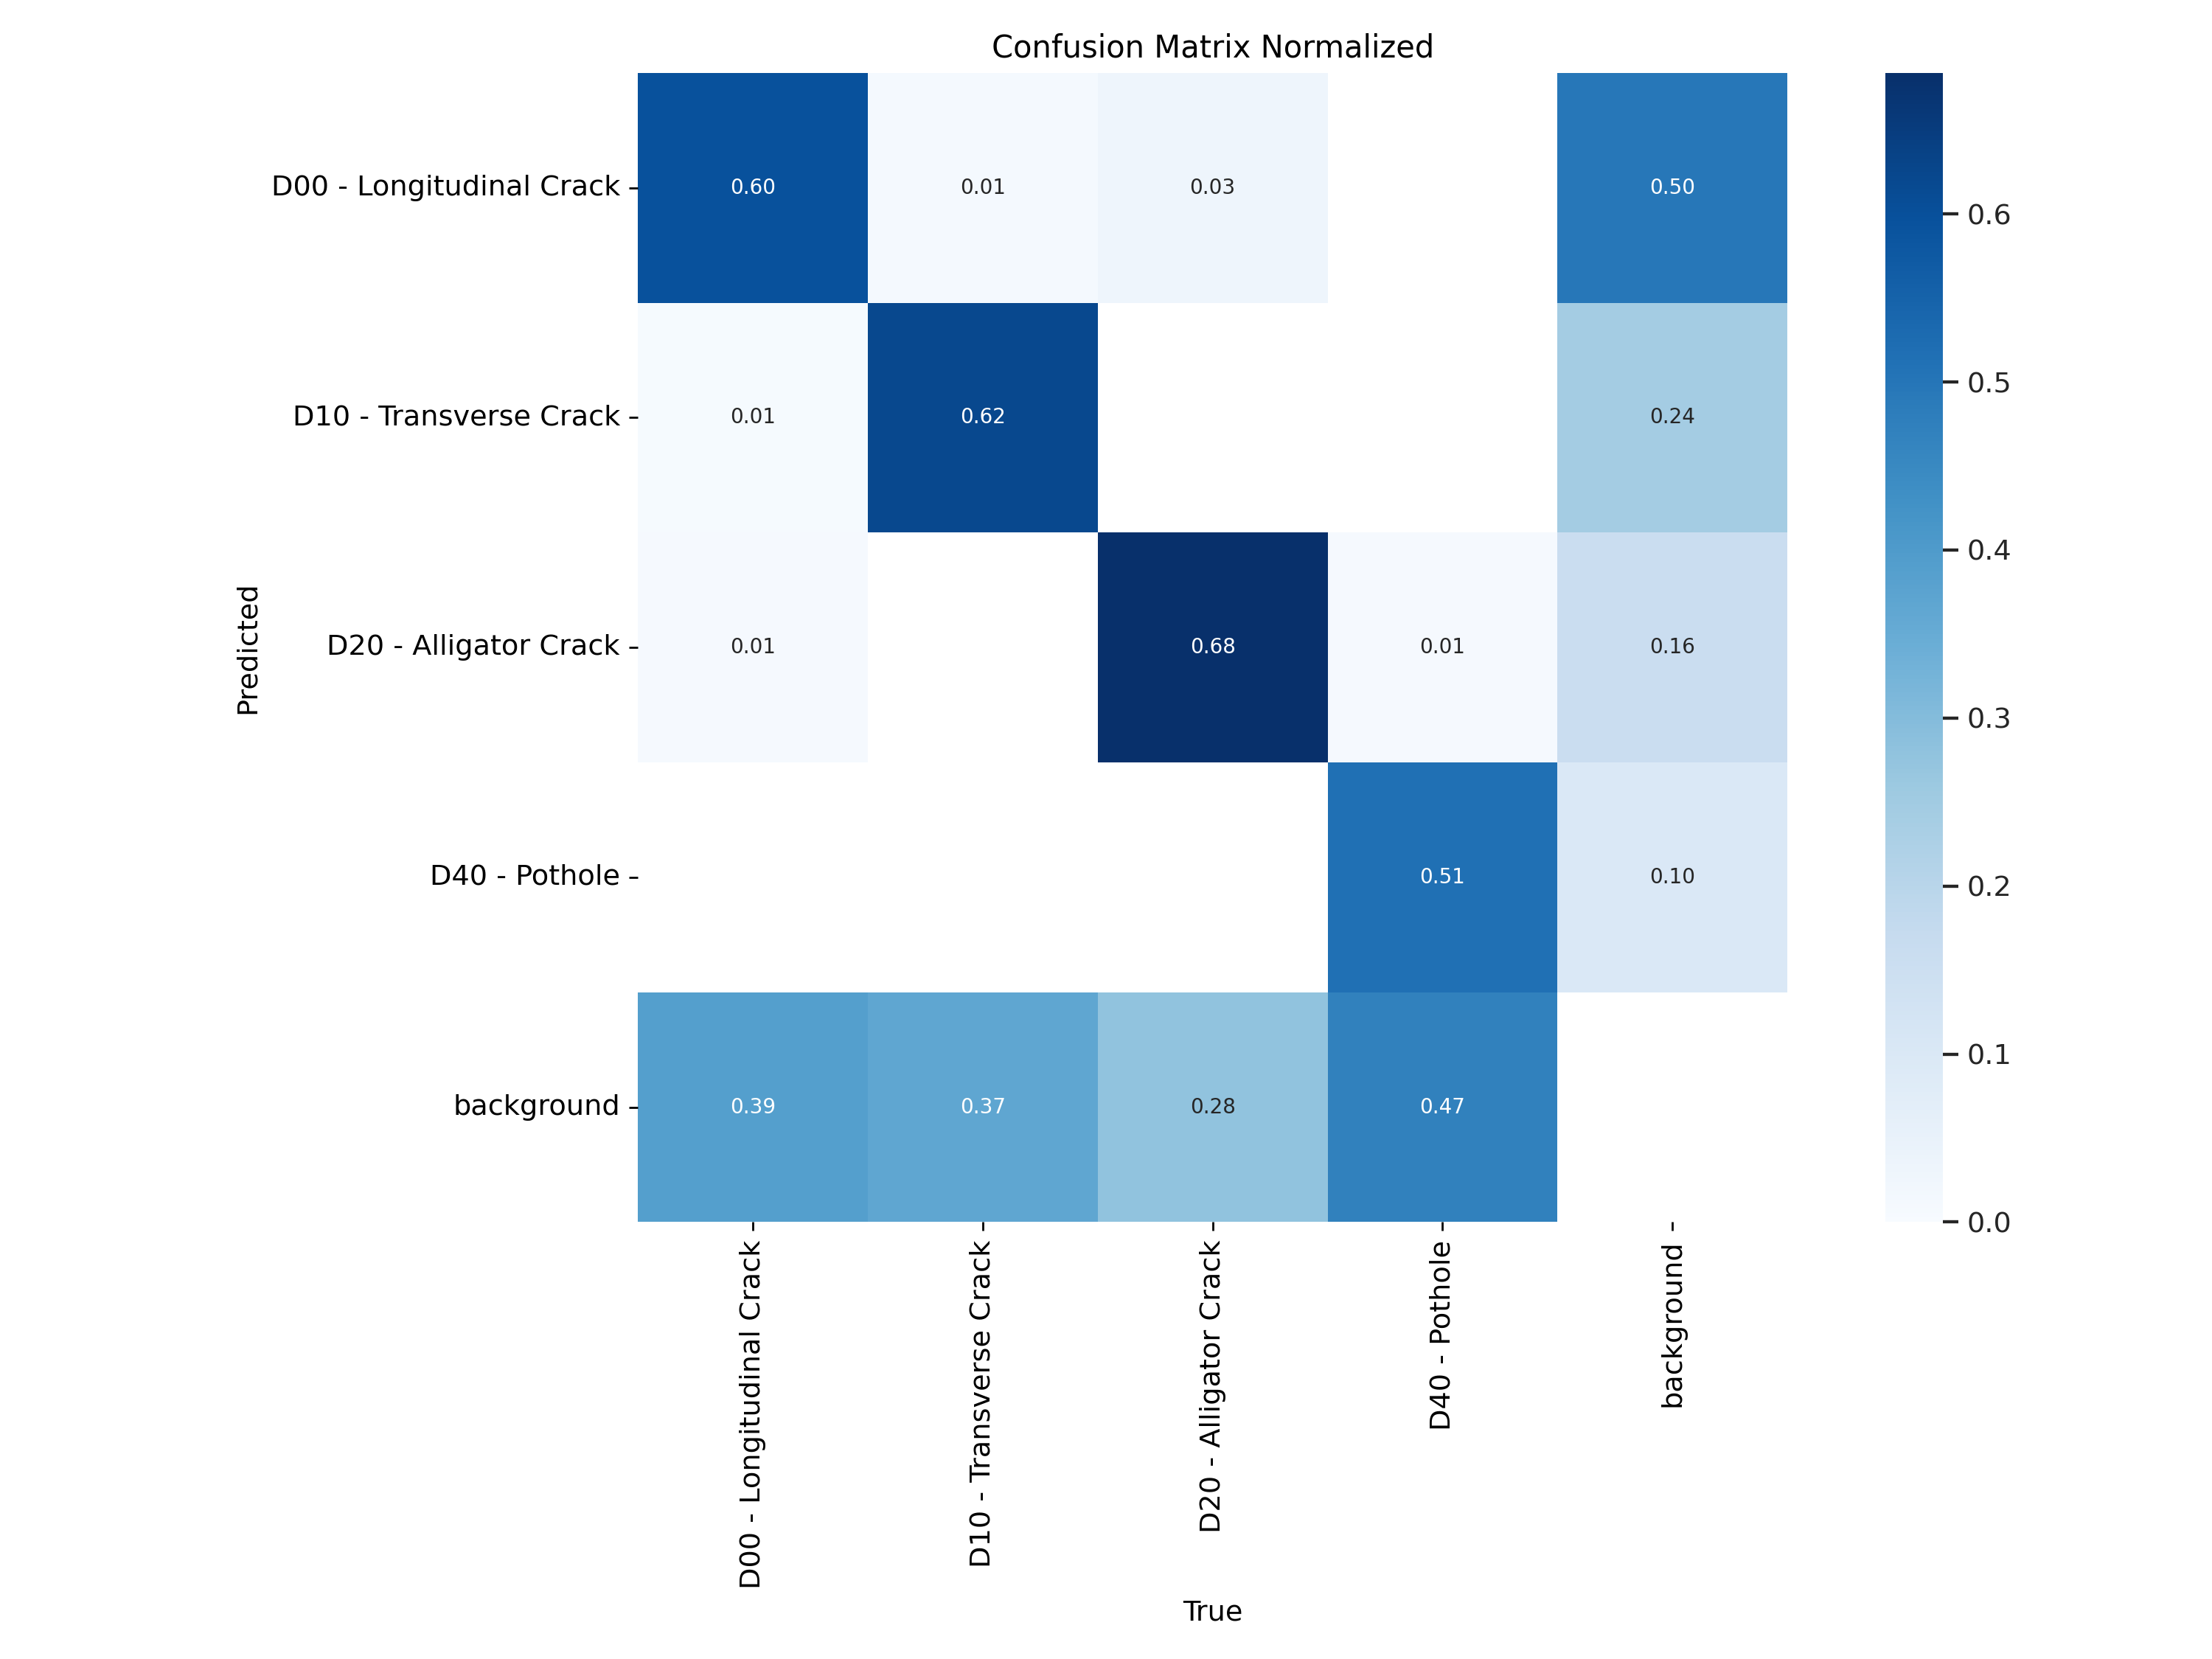
\includegraphics[width=0.45\textwidth]{../img/exp3-val0-all-confusion_matrix_normalized.png}
        \label{fig:exp3_val0_all_confusion_matrix_normalized}
    }
    \subfigure[Matriz de confusión.]{
        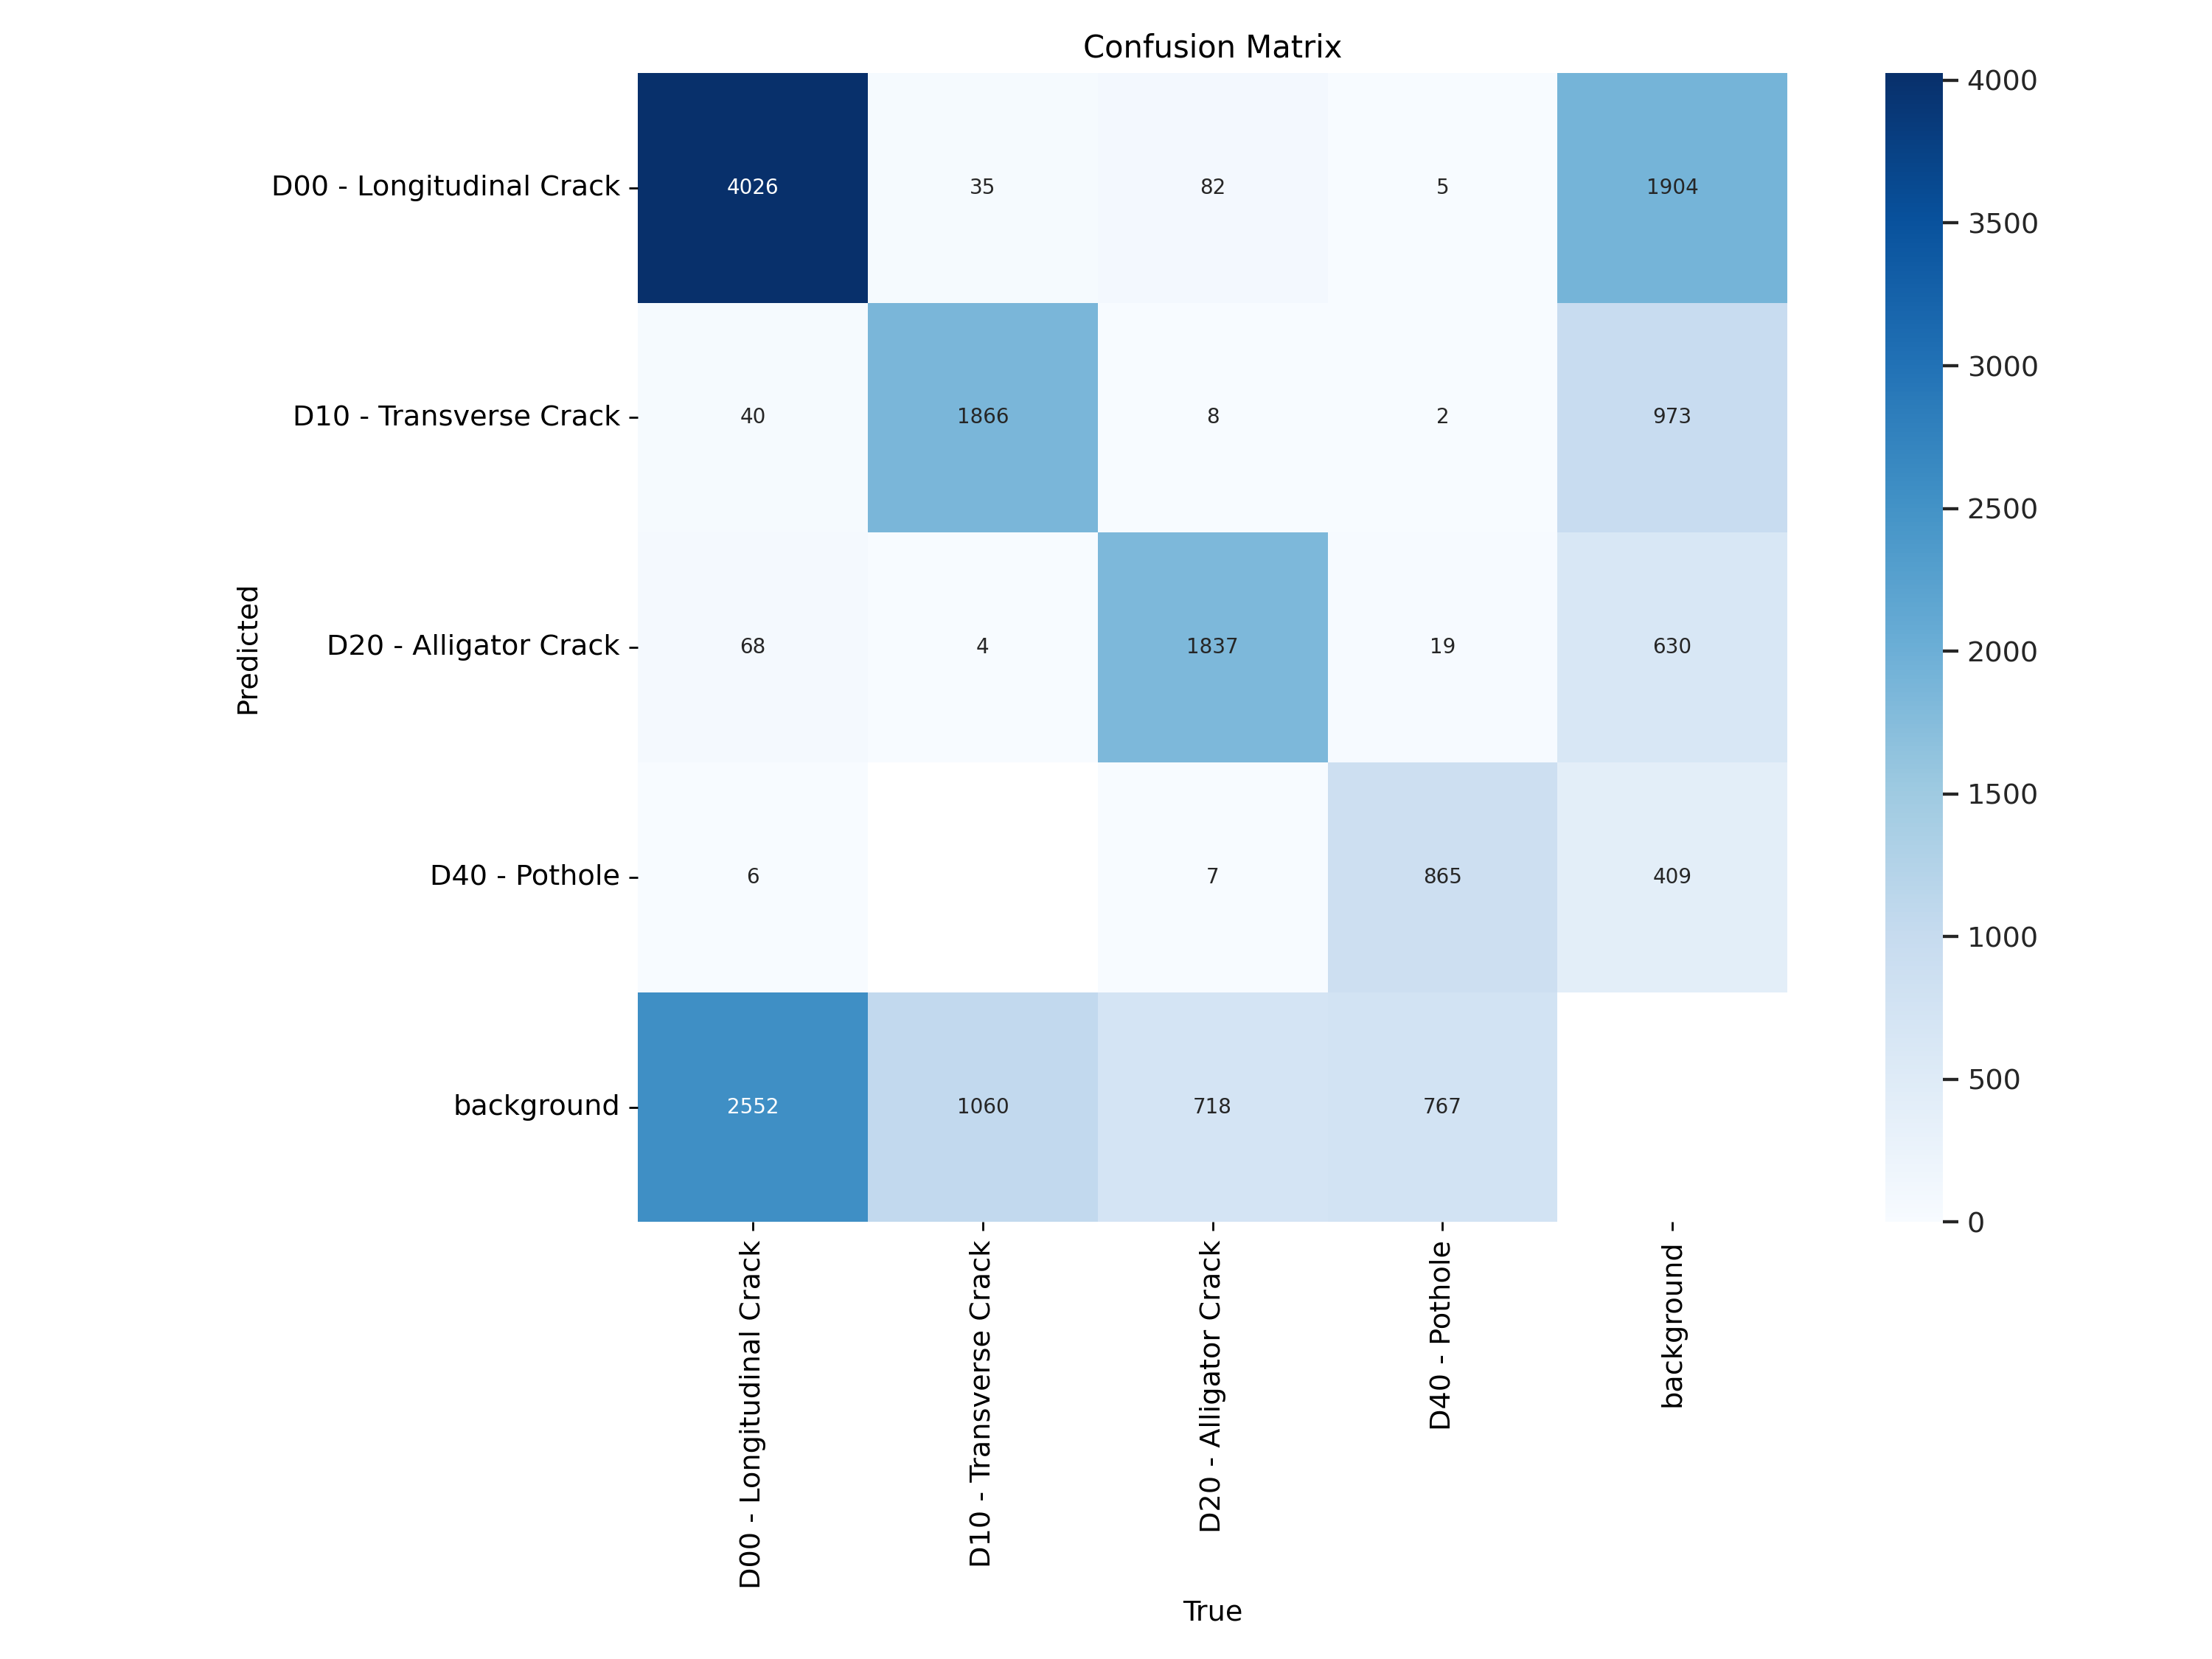
\includegraphics[width=0.45\textwidth]{../img/exp3-val0-all-confusion_matrix.png}
        \label{fig:exp3_val0_all_confusion_matrix}
    }
    \caption{Matrices de confusión de la validación del modelo del experimento 3 sobre los datos de \textit{fold\_0} de todos los conjuntos de datos.}
    \label{fig:exp3_val0_all_confusion_matrices}
\end{figure}

% Añadimos ../img/exp3-val0-india-confusion_matrix_normalized.png, ../img/exp3-val0-japan-confusion_matrix_normalized.png, ../img/exp3-val0-norway-confusion_matrix_normalized.png, ../img/exp3-val0-usa-confusion_matrix_normalized.png como figura de subfiguras 2x2
\begin{figure}[H]
    \centering
    \subfigure[India.]{
        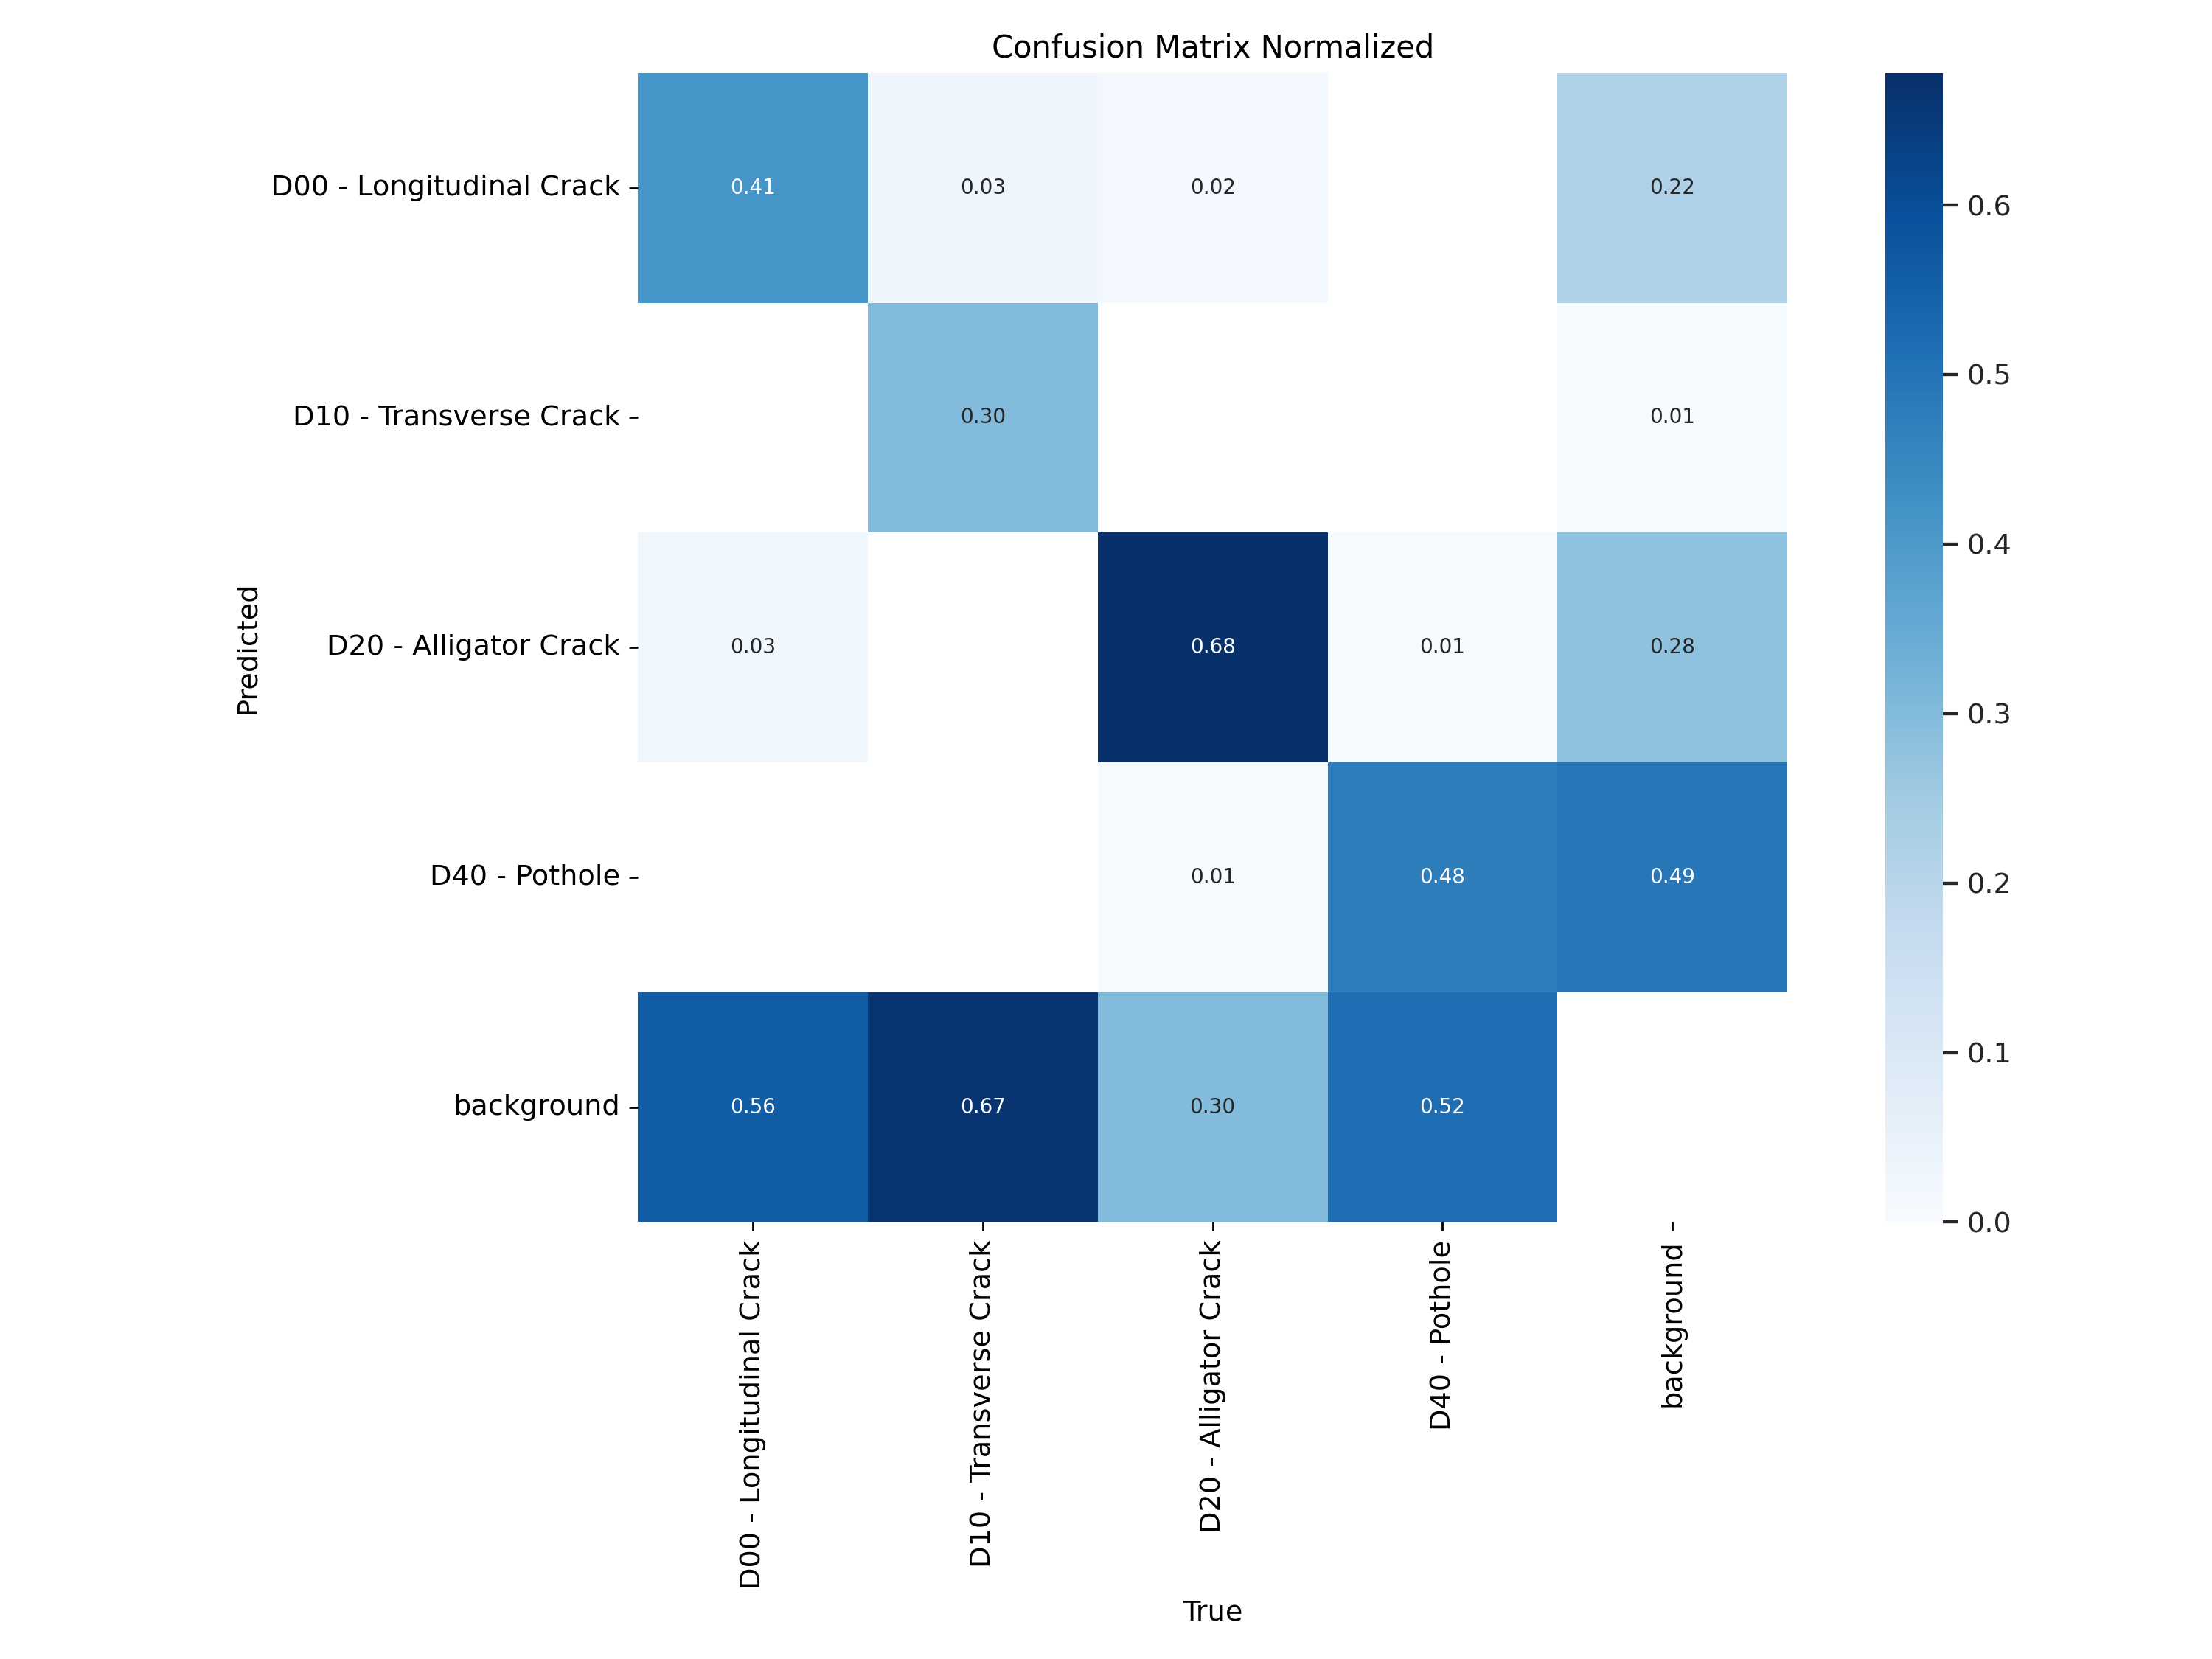
\includegraphics[width=0.45\textwidth]{../img/exp3-val0-india-confusion_matrix_normalized.png}
        \label{fig:exp3_val0_india_confusion_matrix_normalized}
    }
    \subfigure[Japón.]{
        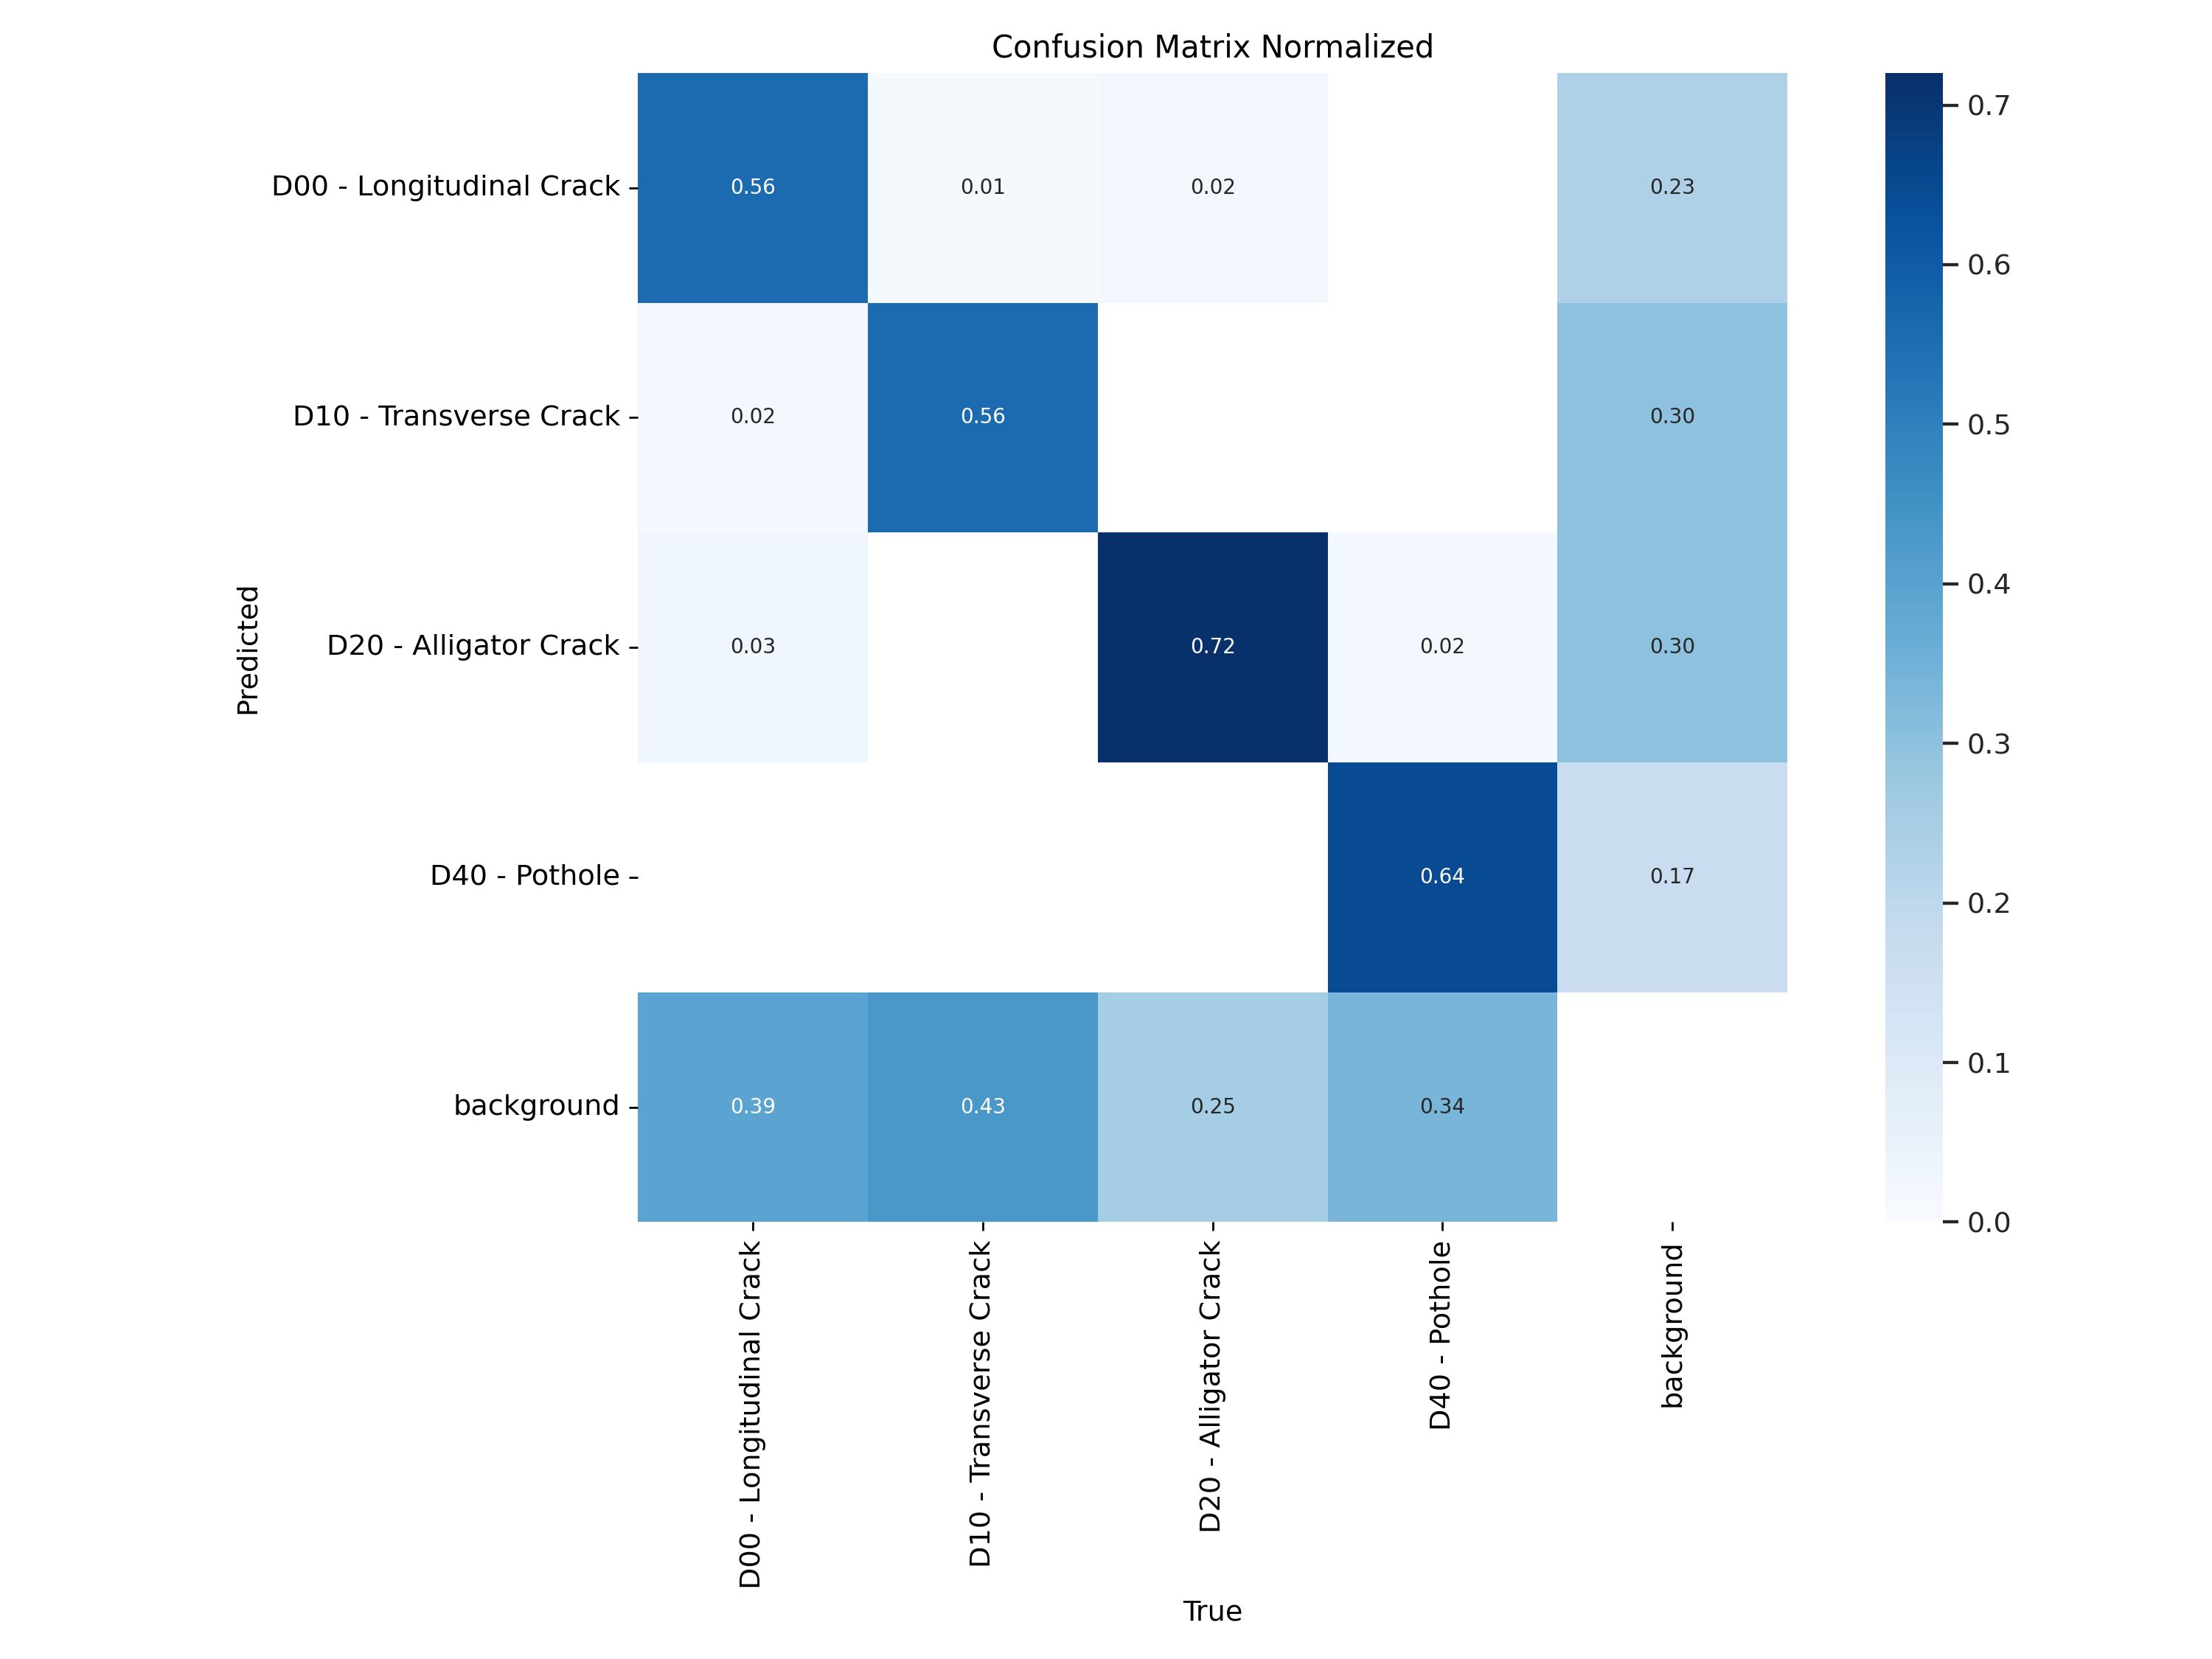
\includegraphics[width=0.45\textwidth]{../img/exp3-val0-japan-confusion_matrix_normalized.png}
        \label{fig:exp3_val0_japan_confusion_matrix_normalized}
    }
    \vskip\baselineskip
    \subfigure[Noruega.]{
        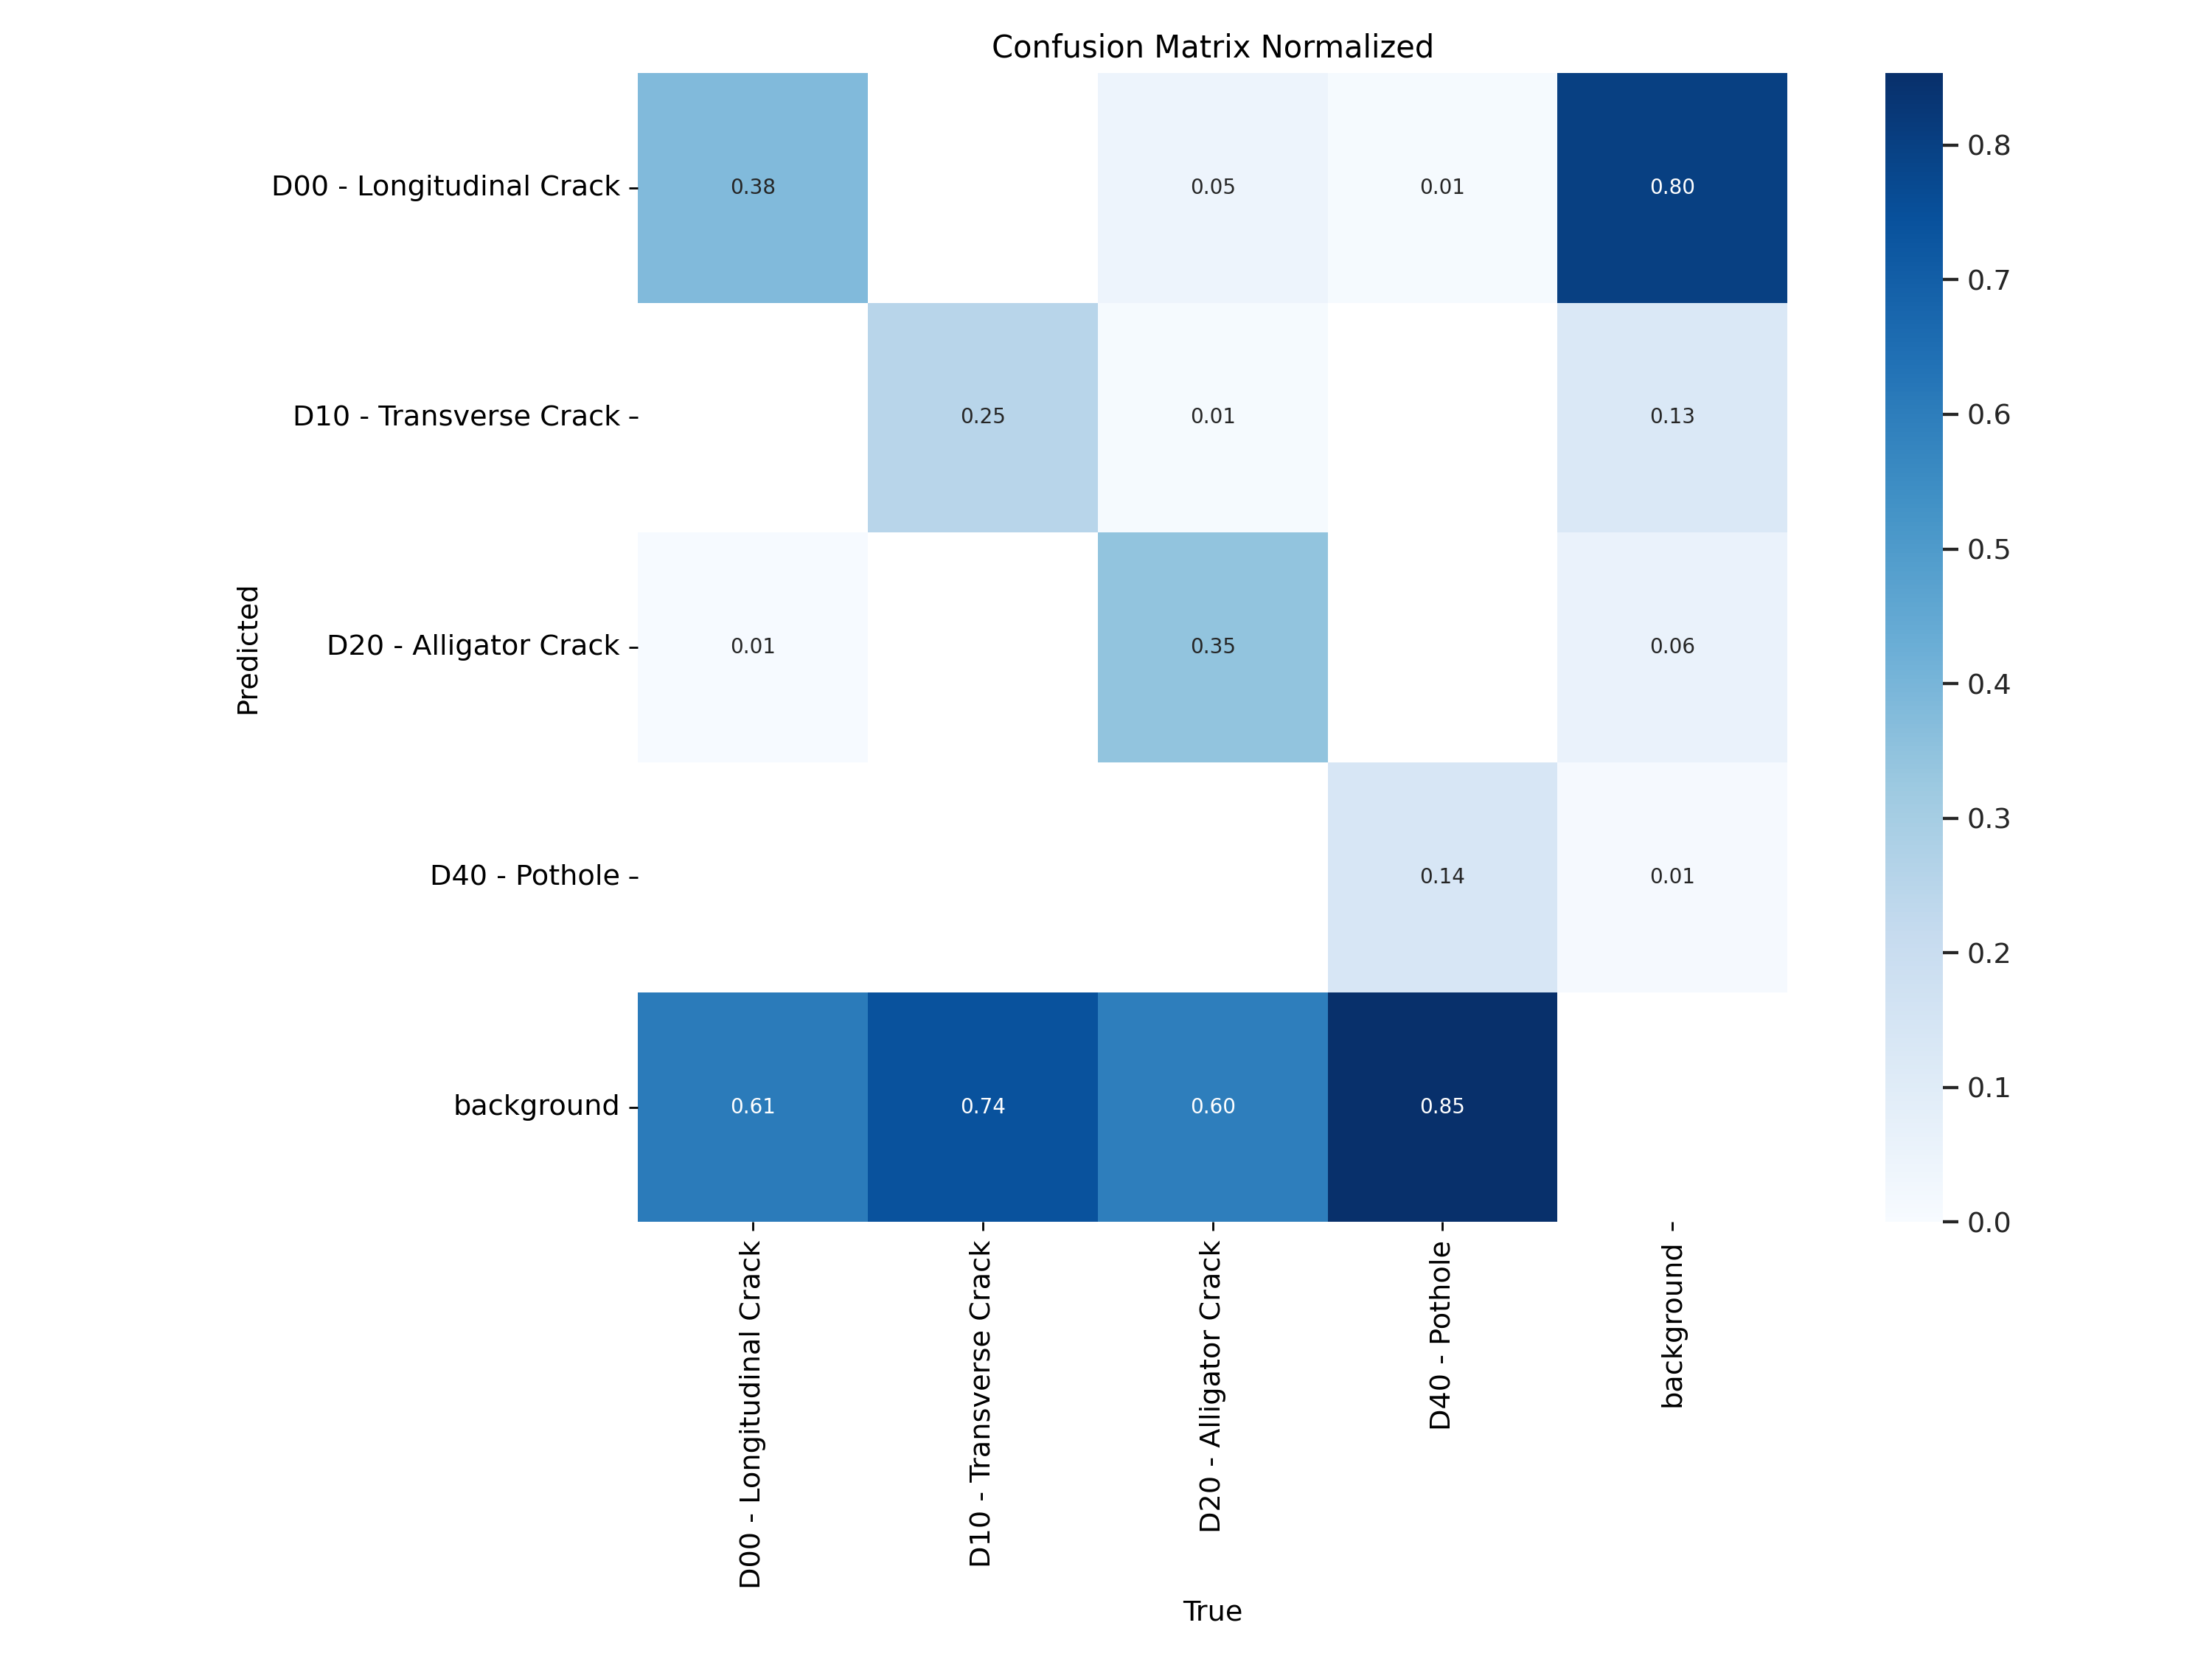
\includegraphics[width=0.45\textwidth]{../img/exp3-val0-norway-confusion_matrix_normalized.png}
        \label{fig:exp3_val0_norway_confusion_matrix_normalized}
    }
    \subfigure[Estados Unidos.]{
        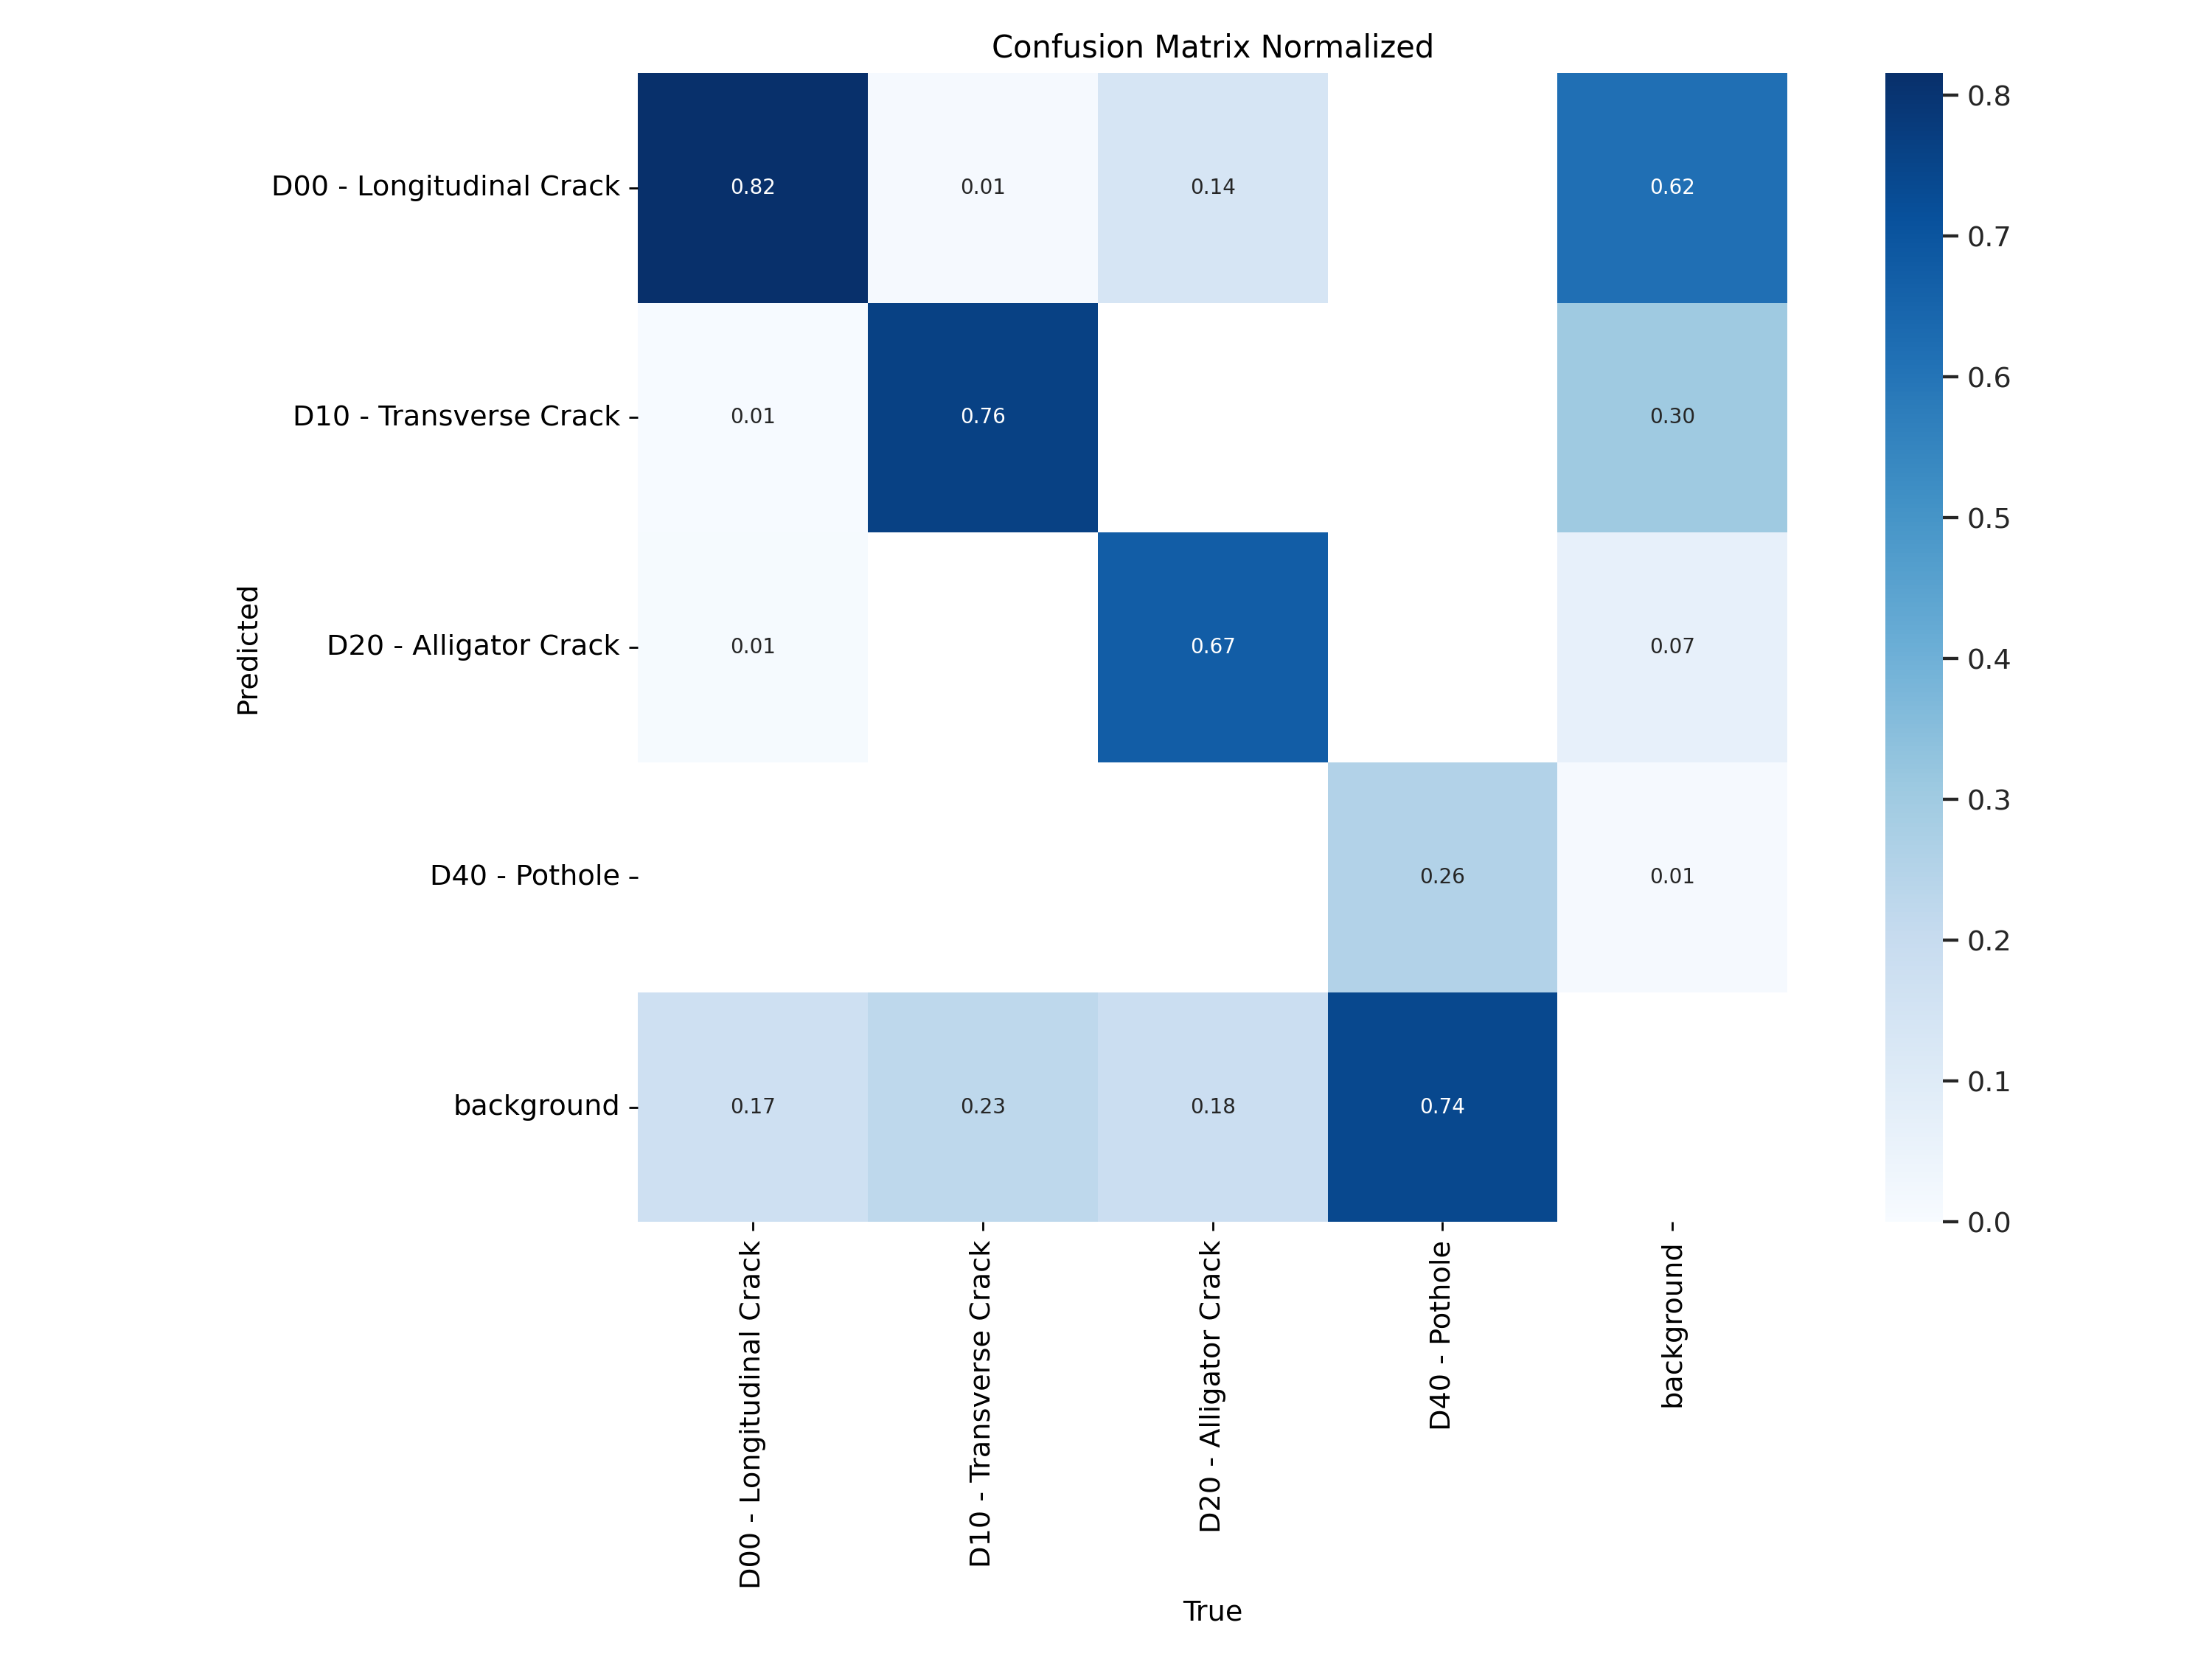
\includegraphics[width=0.45\textwidth]{../img/exp3-val0-usa-confusion_matrix_normalized.png}
        \label{fig:exp3_val0_usa_confusion_matrix_normalized}
    }
    \caption{Matrices de confusión normalizadas de la validación del modelo del experimento 3 sobre los datos de \textit{fold\_0} de los distintos conjuntos de datos.}
    \label{fig:exp3_val0_confusion_matrices_normalized}
\end{figure}

% Añadimos ../img/exp3-val0-india-confusion_matrix.png, ../img/exp3-val0-japan-confusion_matrix.png, ../img/exp3-val0-norway-confusion_matrix.png, ../img/exp3-val0-usa-confusion_matrix.png como figura de subfiguras 2x2
\begin{figure}[H]
    \centering
    \subfigure[India.]{
        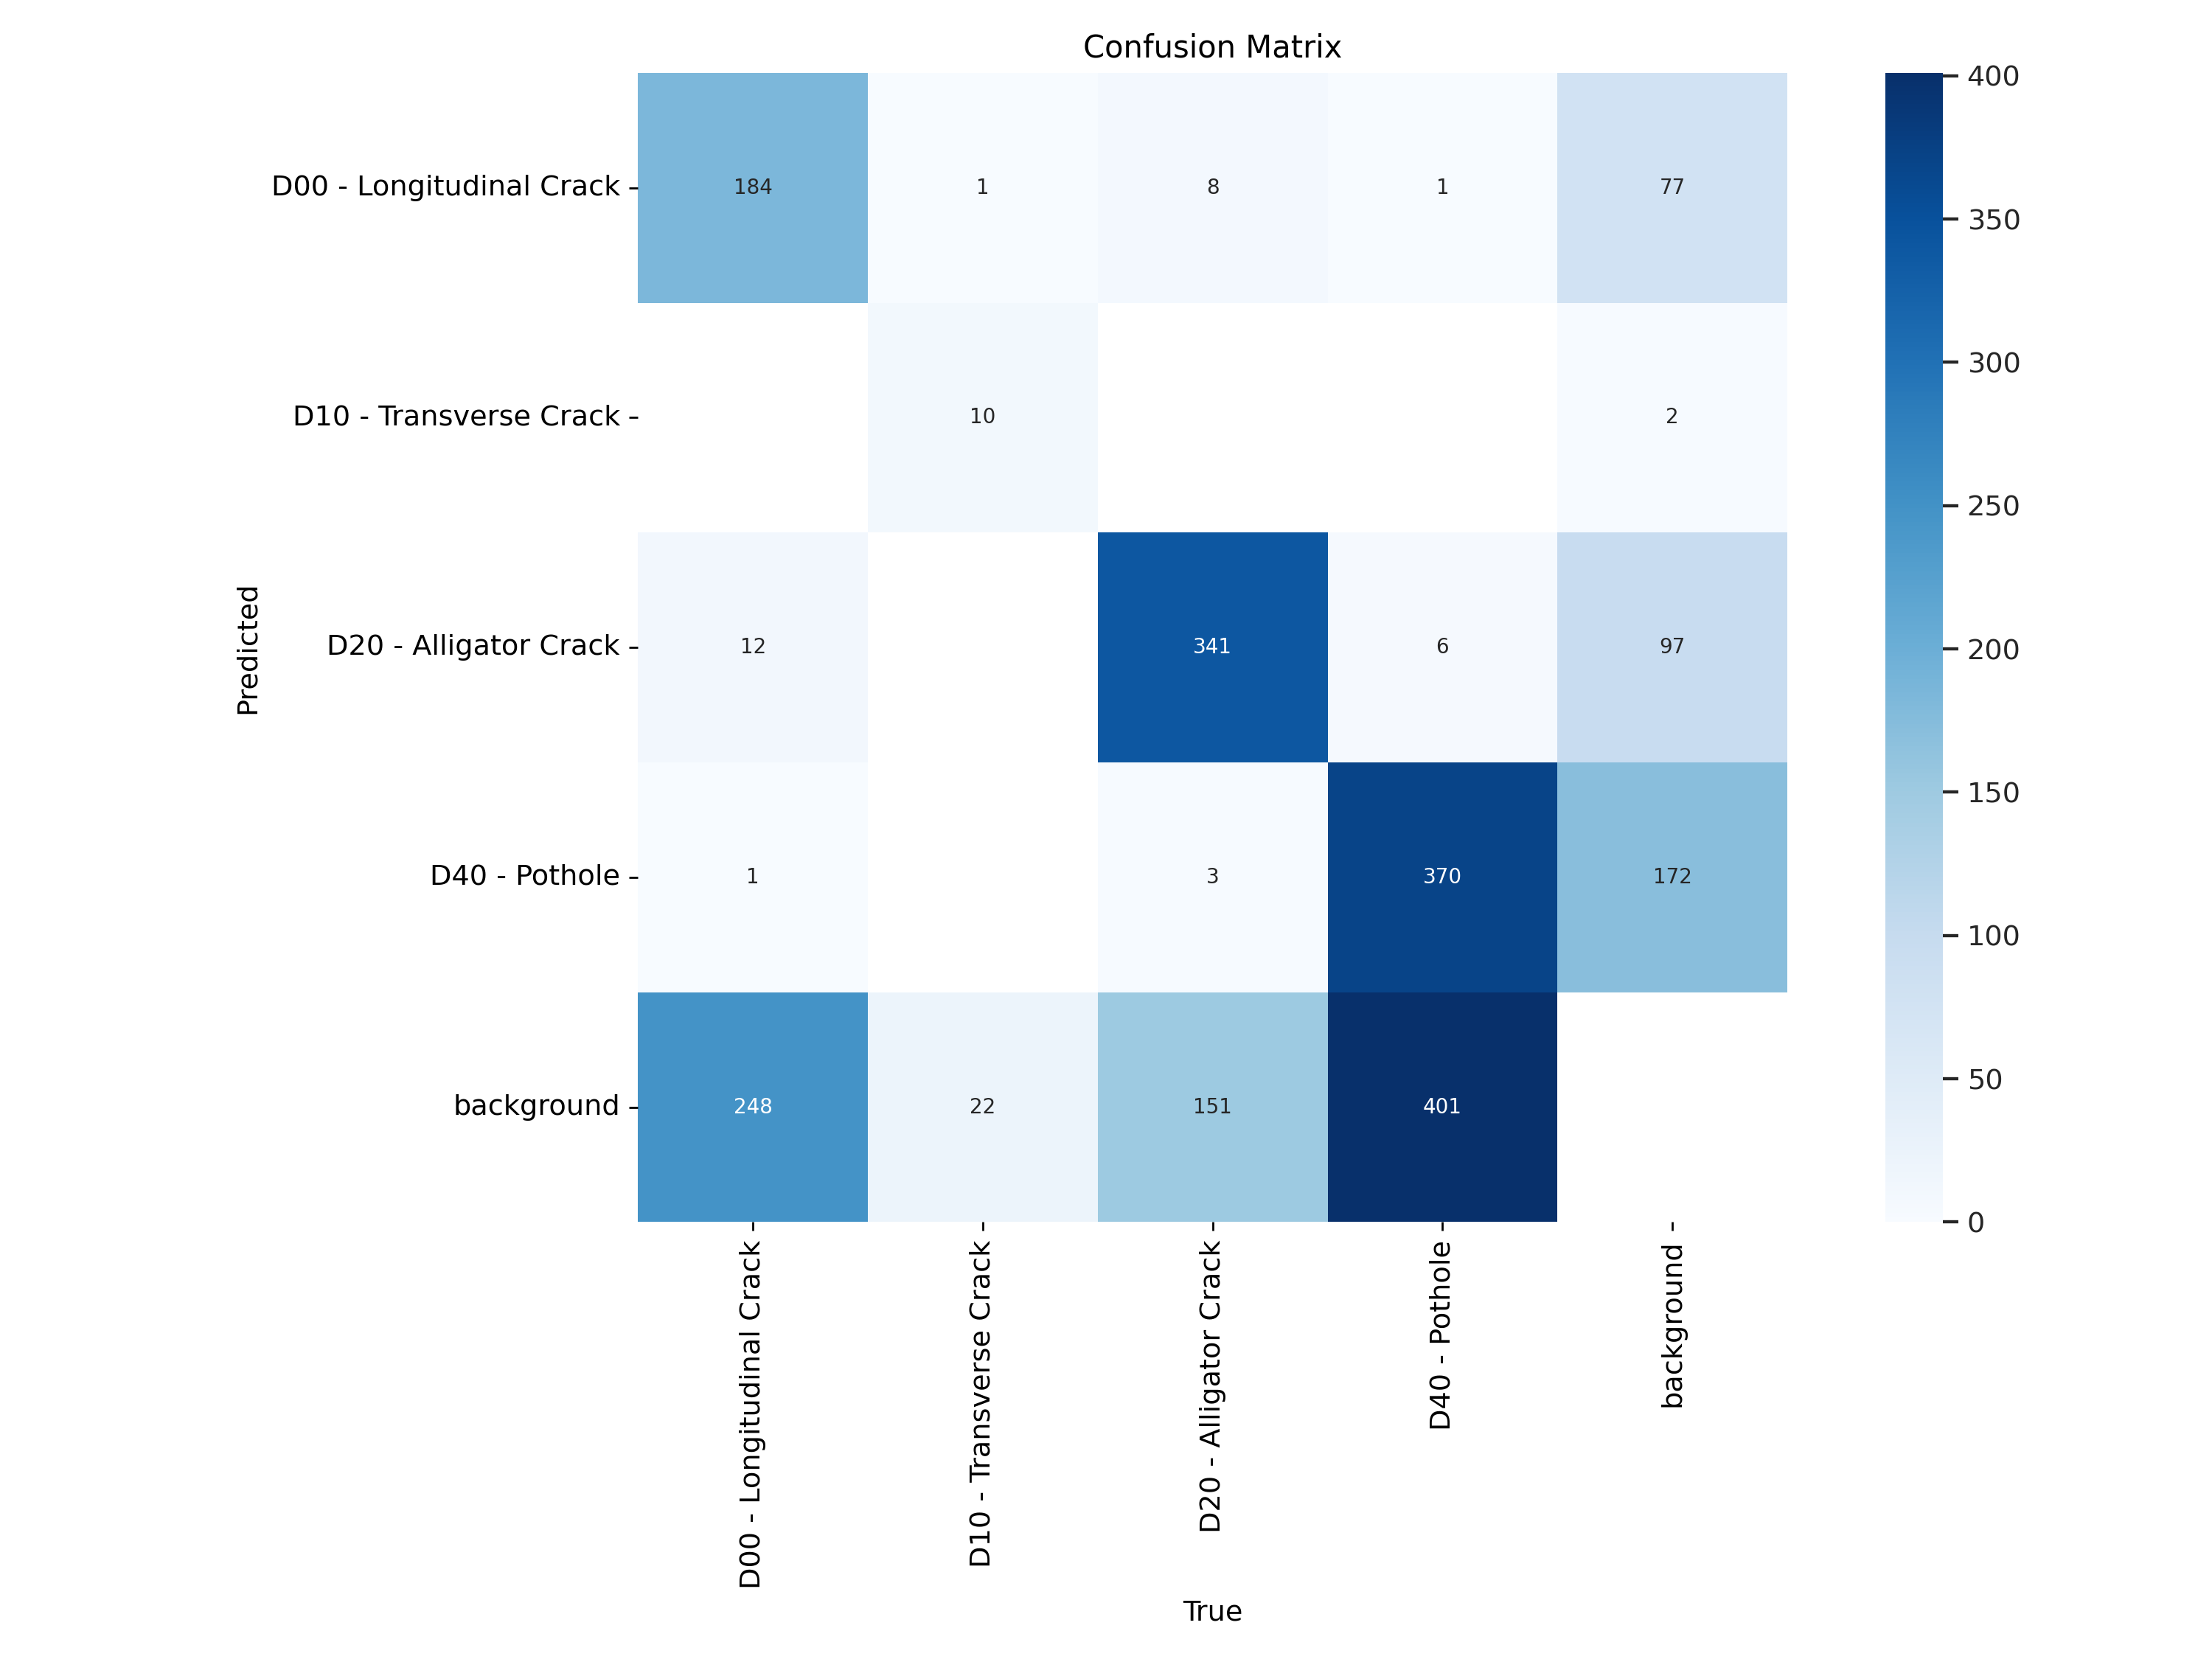
\includegraphics[width=0.45\textwidth]{../img/exp3-val0-india-confusion_matrix.png}
        \label{fig:exp3_val0_india_confusion_matrix}
    }
    \subfigure[Japón.]{
        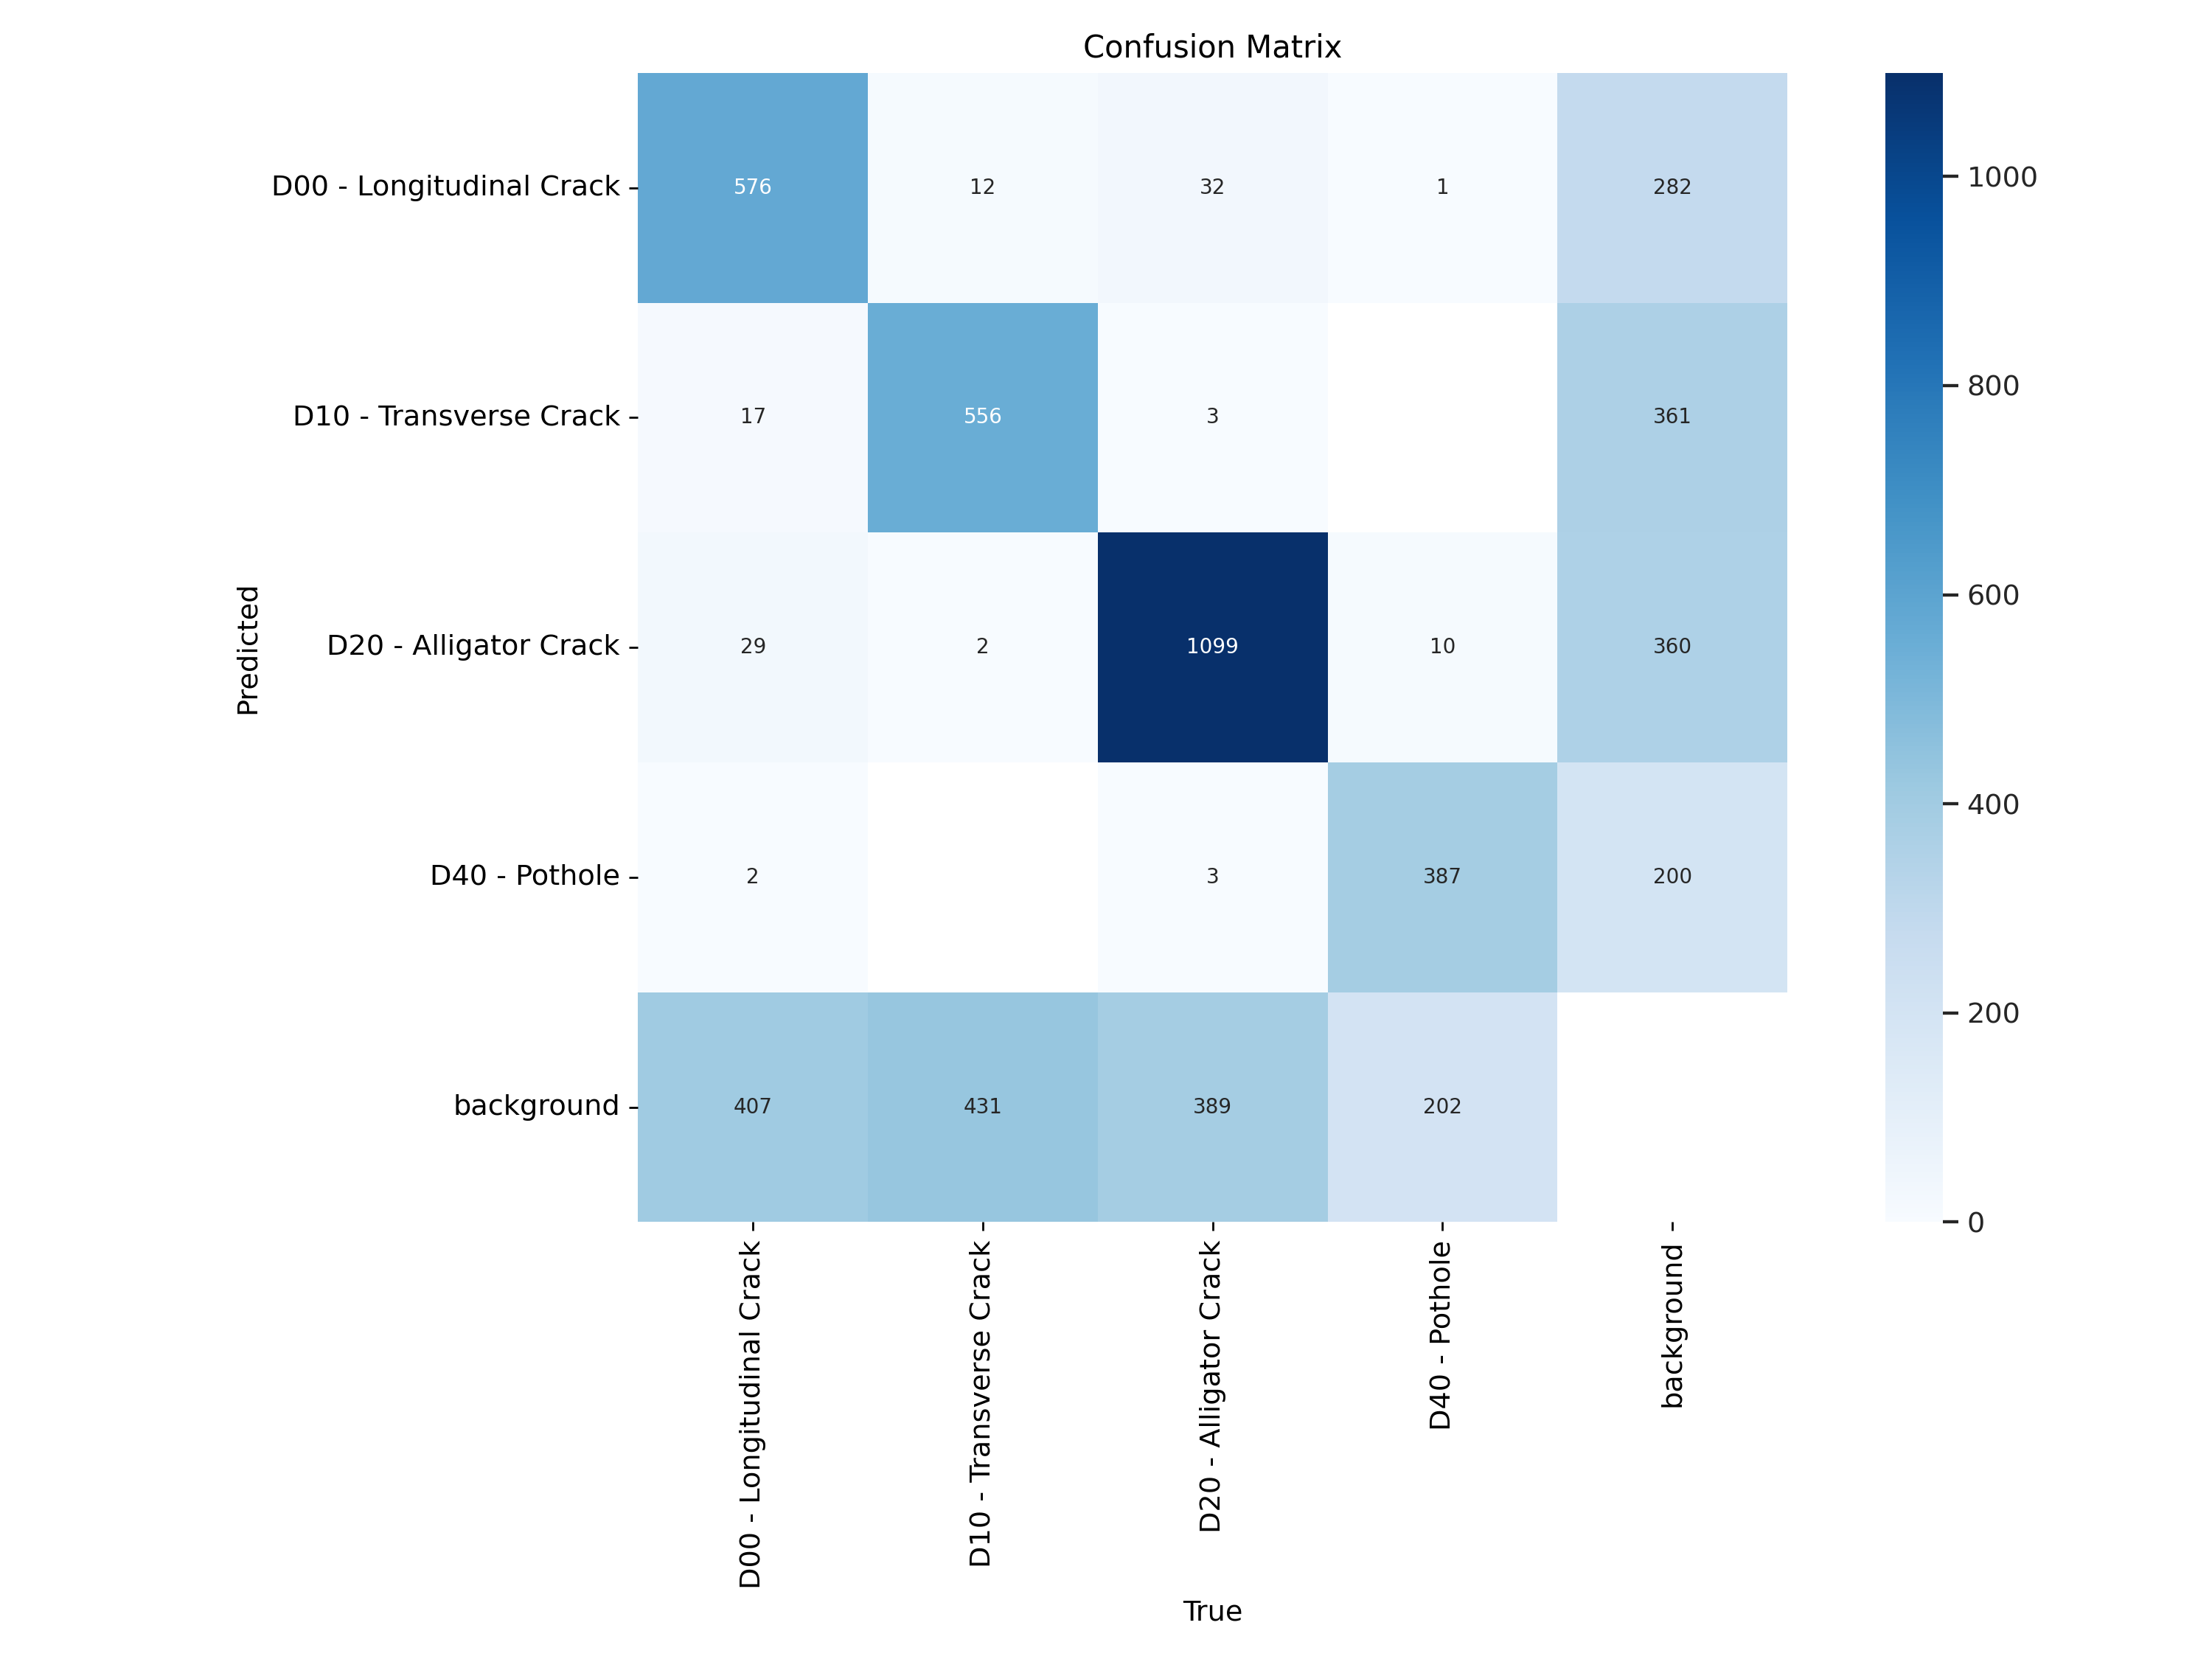
\includegraphics[width=0.45\textwidth]{../img/exp3-val0-japan-confusion_matrix.png}
        \label{fig:exp3_val0_japan_confusion_matrix}
    }
    \vskip\baselineskip
    \subfigure[Noruega.]{
        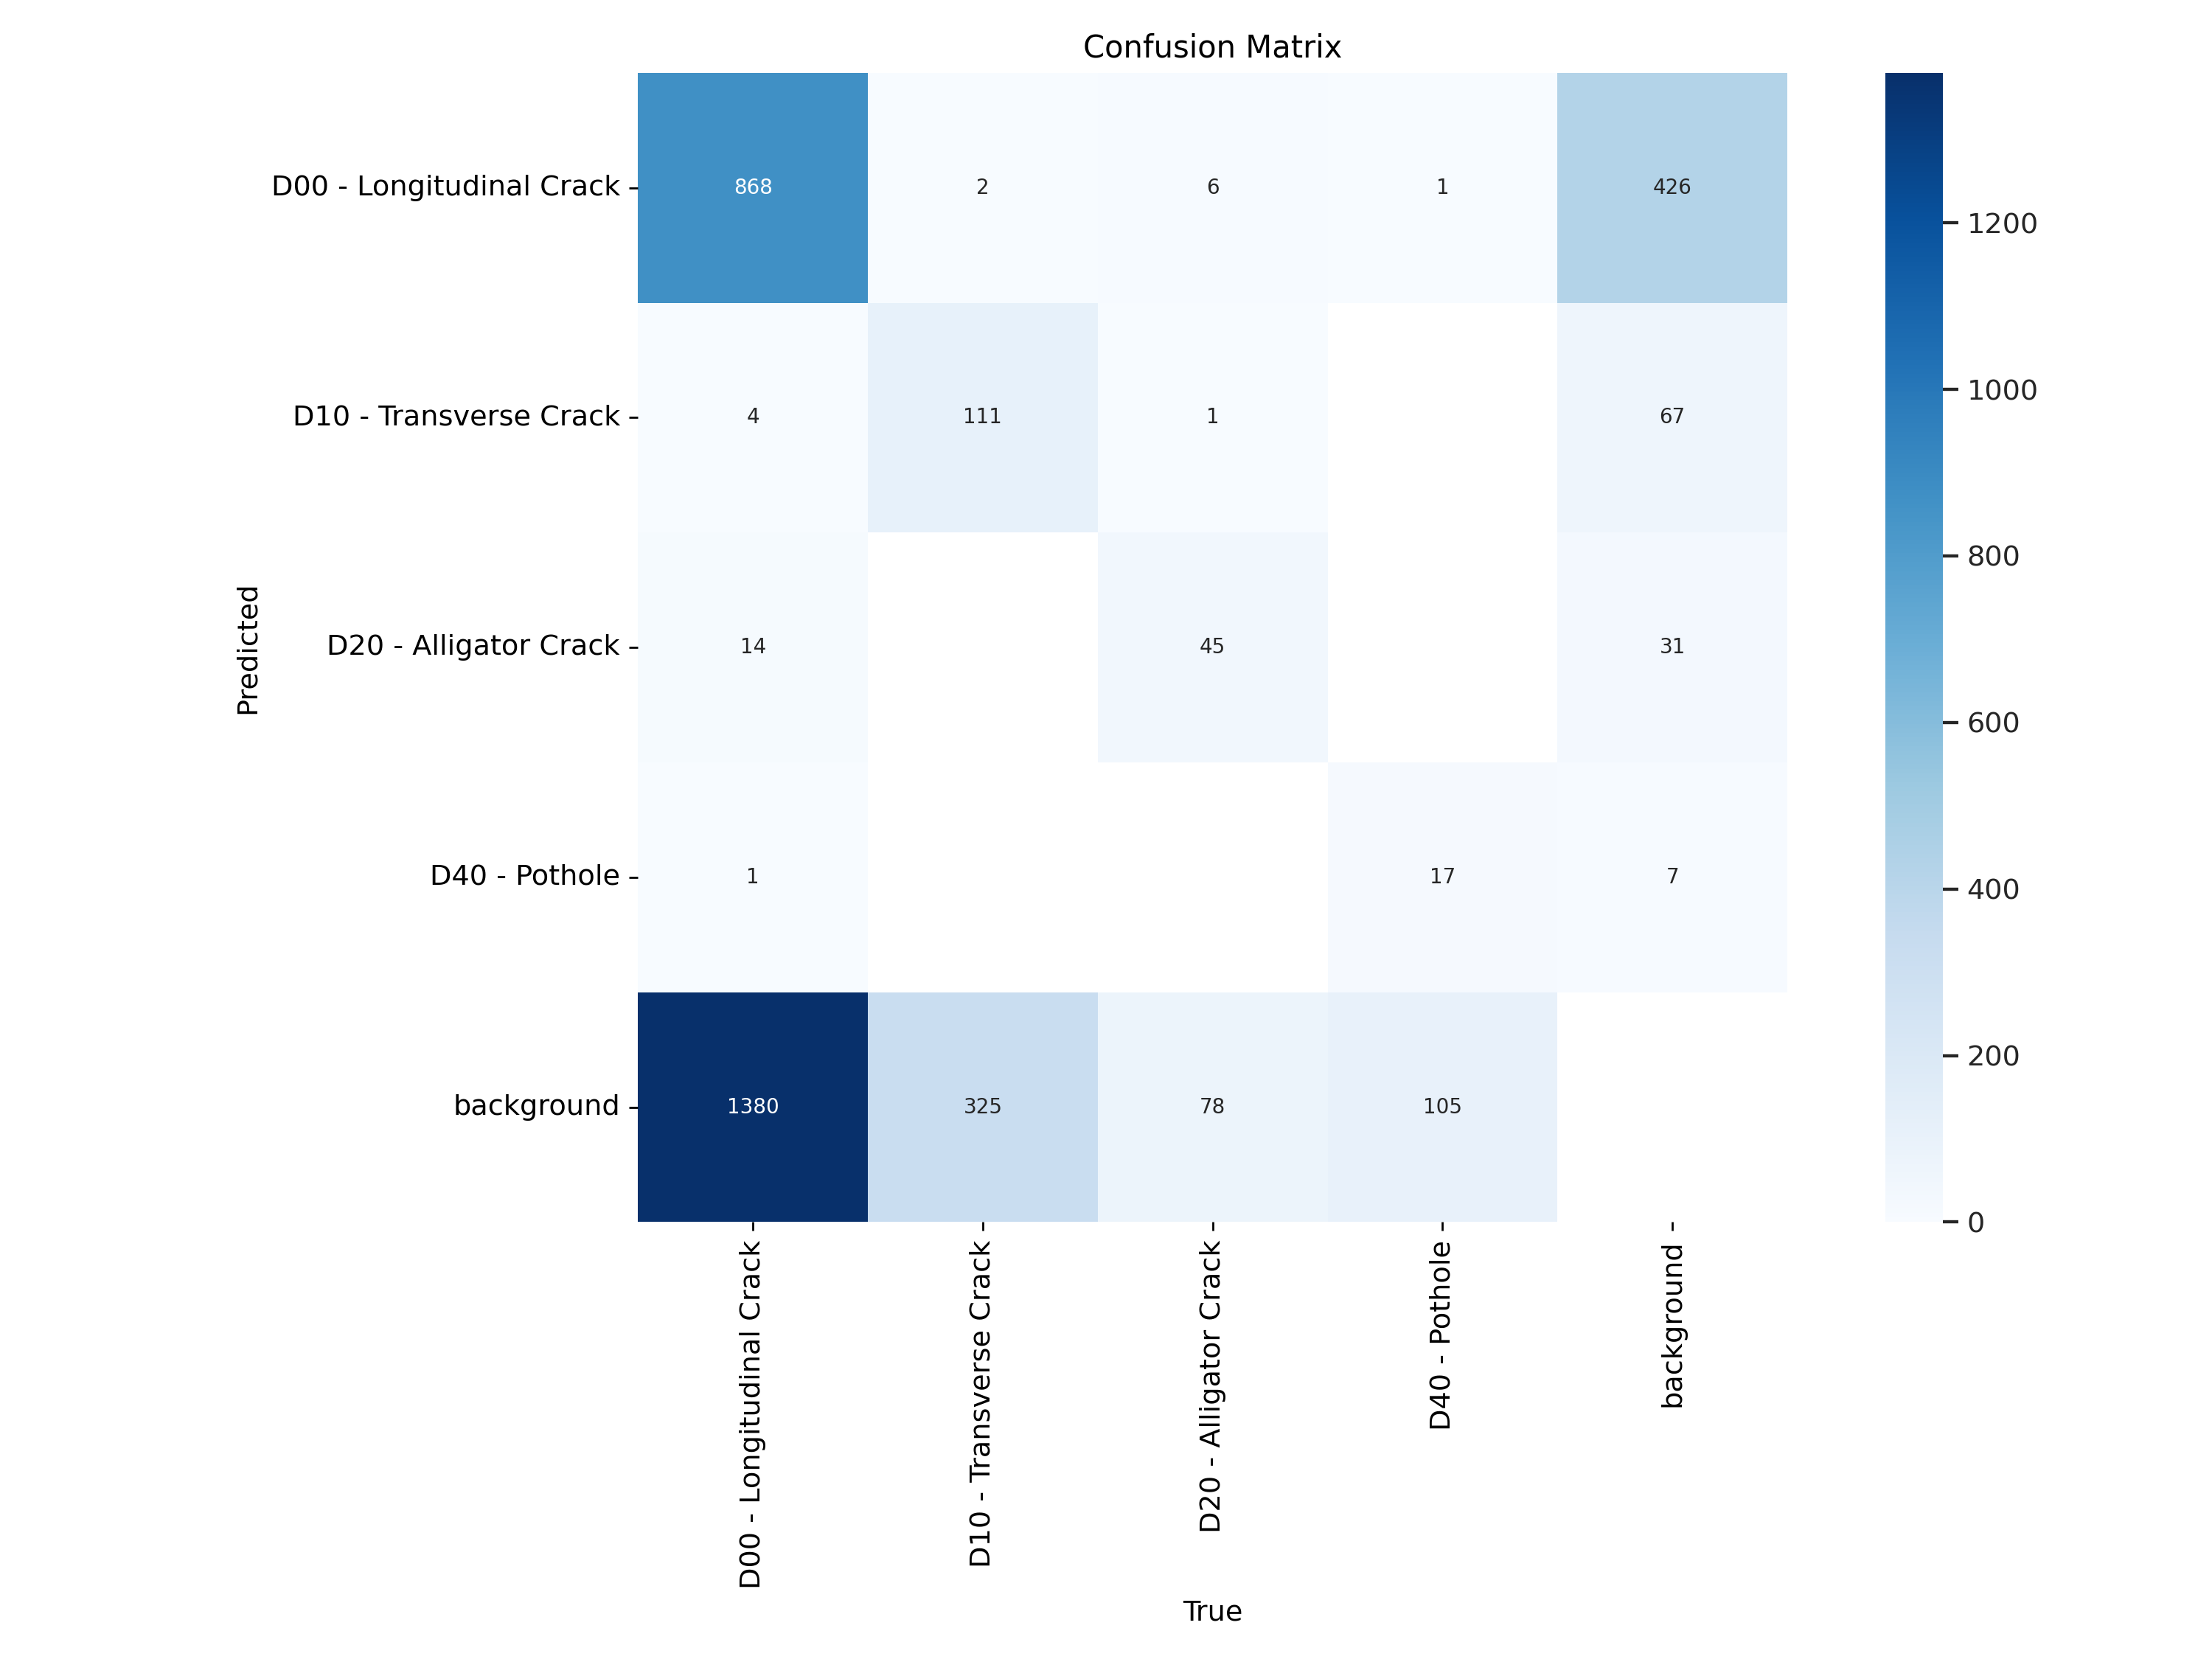
\includegraphics[width=0.45\textwidth]{../img/exp3-val0-norway-confusion_matrix.png}
        \label{fig:exp3_val0_norway_confusion_matrix}
    }
    \subfigure[Estados Unidos.]{
        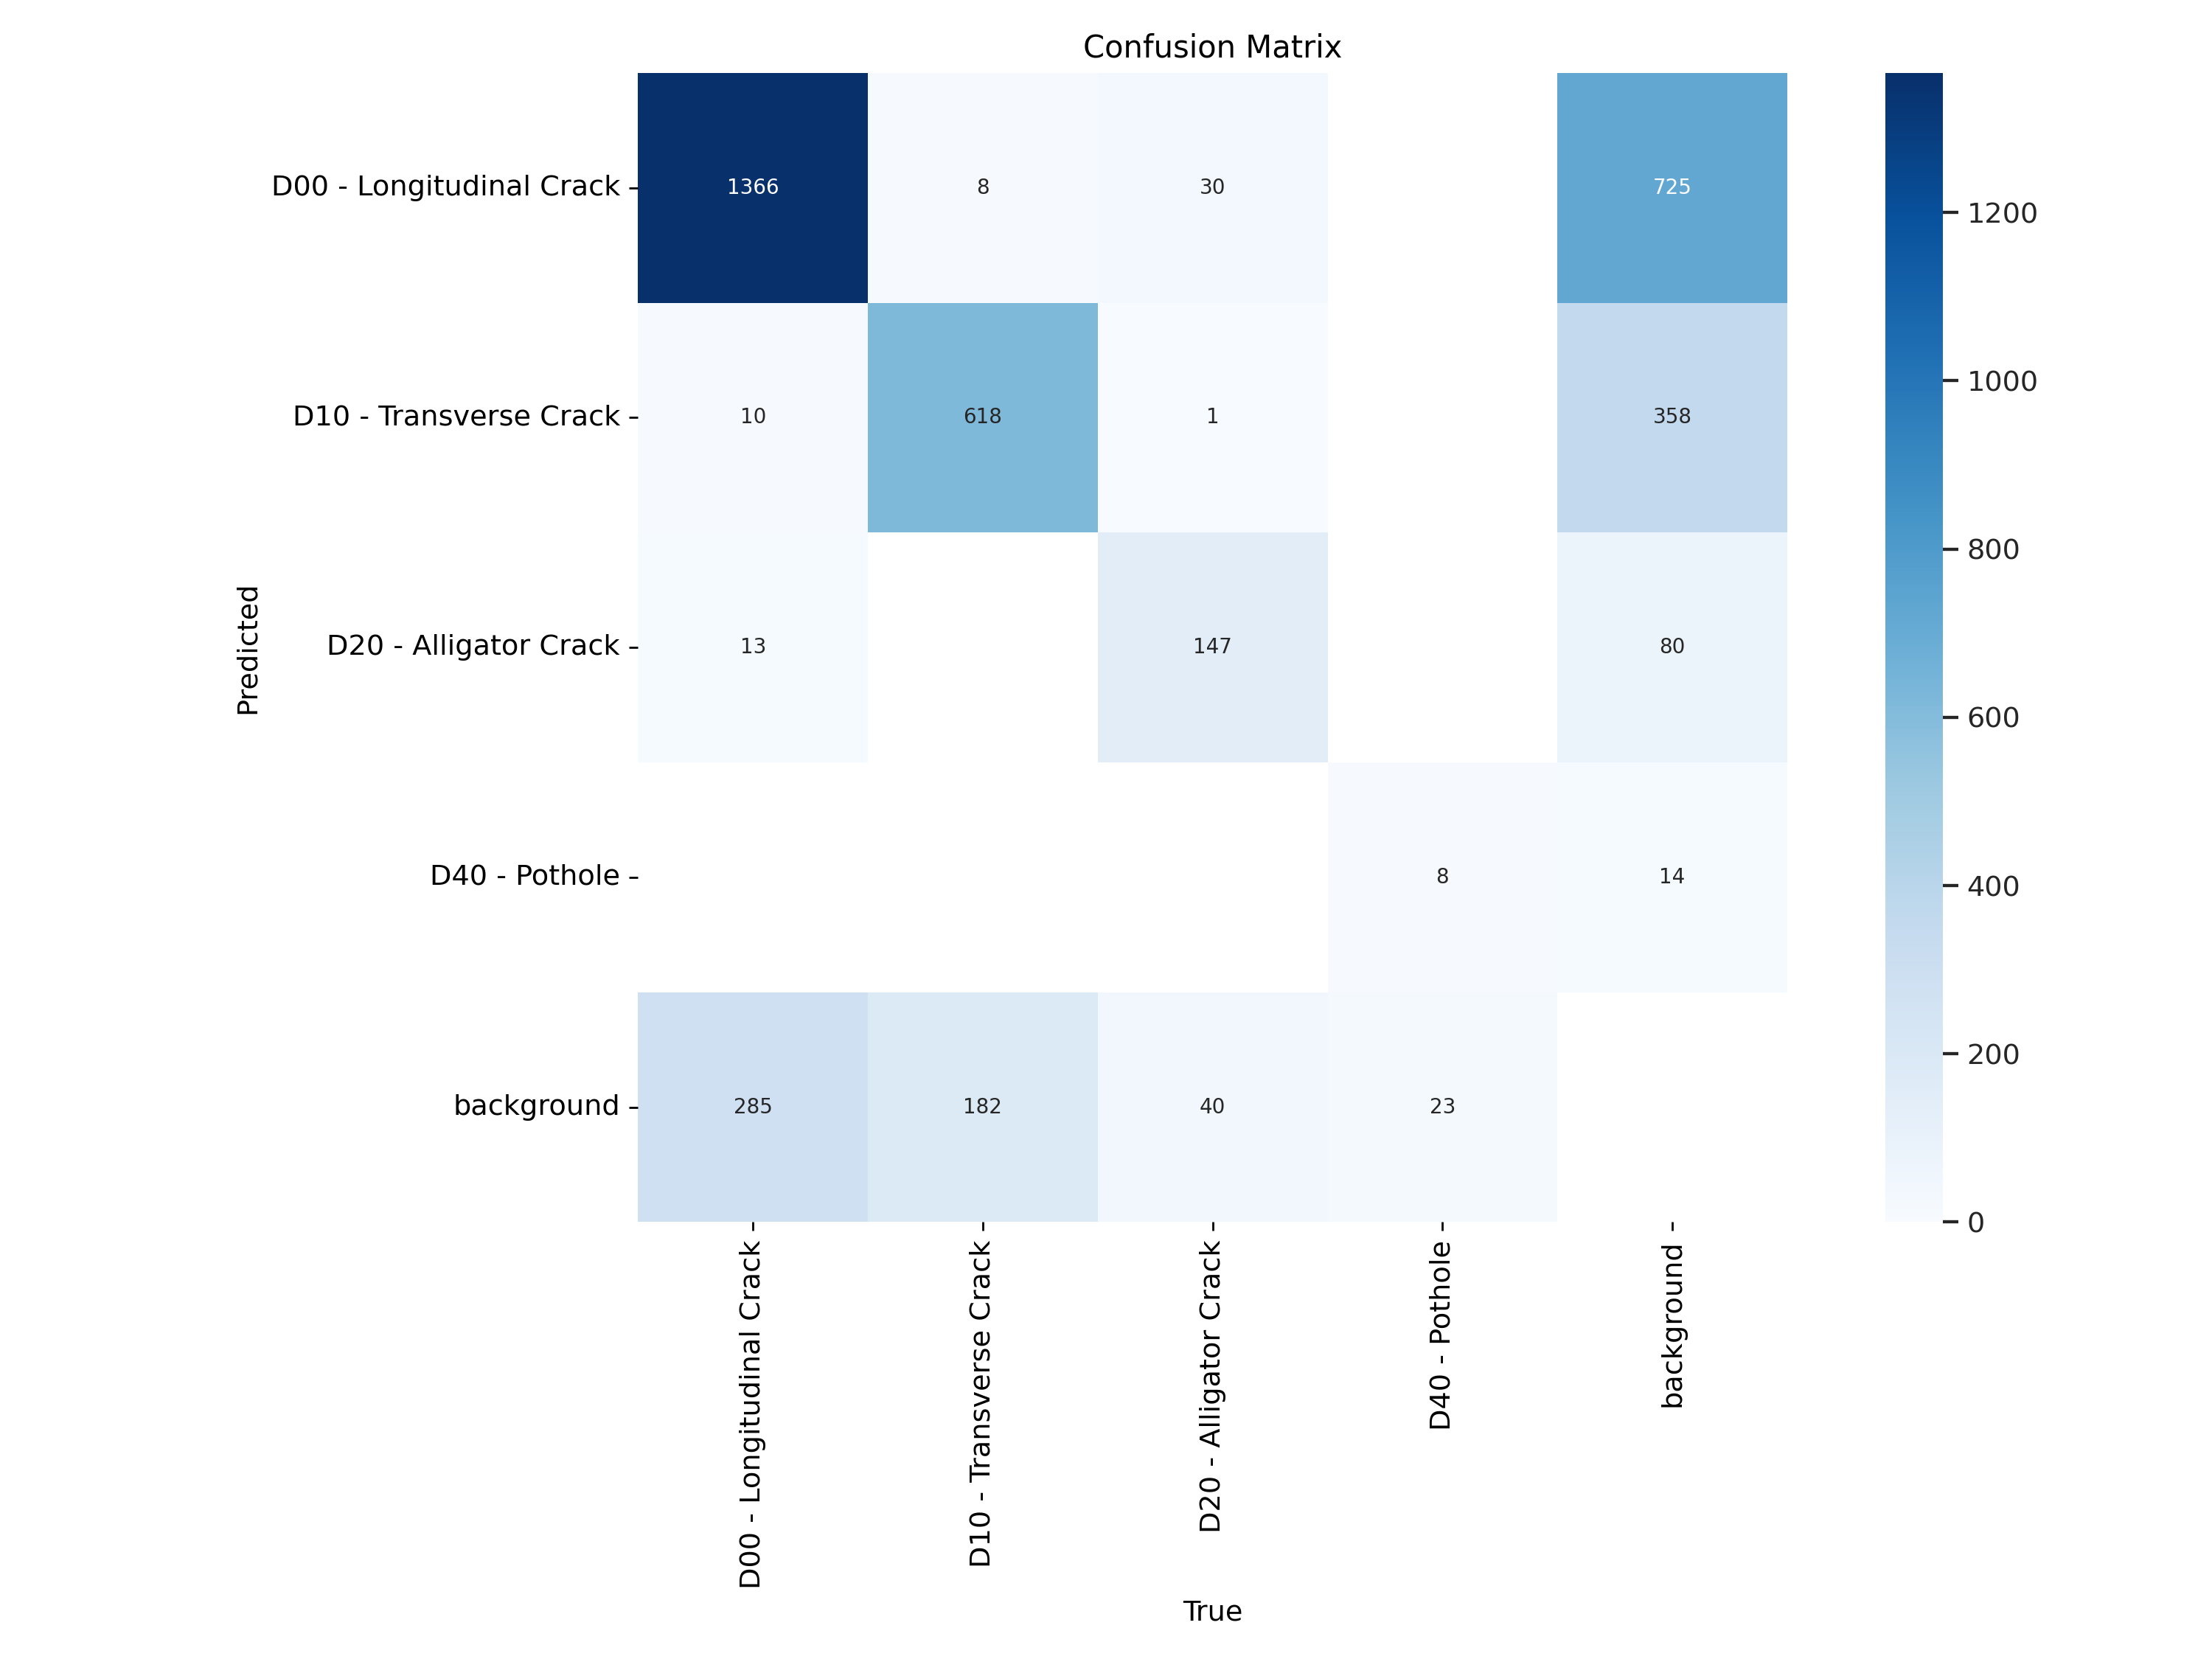
\includegraphics[width=0.45\textwidth]{../img/exp3-val0-usa-confusion_matrix.png}
        \label{fig:exp3_val0_usa_confusion_matrix}
    }
    \caption{Matrices de confusión de la validación del modelo del experimento 3 sobre los datos de \textit{fold\_0} de los distintos conjuntos de datos.}
    \label{fig:exp3_val0_confusion_matrices}
\end{figure}